\documentclass[english]{article}
\usepackage[english]{babel}
\usepackage[T1]{fontenc}

\usepackage[utf8]{inputenc}
% OR for using utf8x
%\usepackage{ucs}
%\usepackage[utf8x]{inputenc}

\usepackage{float}
\usepackage{graphicx} % FOR final compile
%\usepackage[draft]{graphicx} % doesn't draw / load the images every compile

\makeatletter
\usepackage[a4paper,top=2cm,bottom=2cm,left=2cm,right=2cm]{geometry}
\usepackage{enumitem}
\usepackage{subfig}
\usepackage{amsthm}
\usepackage{amsmath}
\usepackage{epstopdf}
\usepackage{fancyhdr}
\usepackage{booktabs,array}

\hyphenation{english}
\makeatother

\usepackage{babel}

\usepackage{listings}
\usepackage{xcolor} % for setting colors
\usepackage{soul} % for text highlighting
\sethlcolor{yellow}

% set the default code style
\lstset{
  frame=tb, % draw a frame at the top and bottom of the code block
  tabsize=4, % tab space width
  breaklines=true, % wrap long code lines instead of overflowing the page
  showstringspaces=false, % don't mark spaces in strings
  numbers=left, % display line numbers on the left
  commentstyle=\color{gray}, % comment color
  keywordstyle=\color{blue}, % keyword color
  stringstyle=\color{red} % string color
}

\begin{document}
\begin{titlepage}

  \begin{center}
    \begin{Large} \textbf{UNIVERSITY OF PADOVA} \\
    \end{Large} \vspace{1cm}
    \vspace{3cm}
    \begin{Large} Embedded Real--Time Control
    \end{Large}
    \par
  \end{center}

  \begin{center}
    \begin{Large}Laboratory 2 report\\ Open-loop control and motor identification\\
    \end{Large}
    \par
  \end{center}

  \begin{center}
    \vspace{2cm}
    \begin{figure}[!htb]
      \centering 
\includegraphics[width=8cm]{figures/unipd-logo.png}\\

    \end{figure}

    \par
  \end{center}

  \begin{center}
    \vspace{2cm}
    {\Large \textbf{Names} -- \textbf{Student ID Numbers}} \\[1em]

    \begin{tabular}{lc}
      Diego Marchini   & 2239741 \\
      Alessio Modonesi & 2244493 \\
      Susanna Sandoyan & 2222159 \\
      Mattia Zanini    & 2239257
    \end{tabular}

    \vspace{2cm}
    {\Large Academic Year 2026-2027}
  \end{center}

\end{titlepage}

\tableofcontents \newpage

\section{Laboratory 2: Open-Loop Control and Motor Identification}
\label{sec:lab2}

In this laboratory we applied voltage steps with a known amplitude to the two DC motors of the TurtleBot, running in
open loop, measured the angular speed with the encoders, and used the step responses to estimate a first-order model
of each motor. The models were then used to tune the PI controller needed in Laboratory~3.

\subsection{Relevant theoretical notions}
\label{sec:lab2-theory}

\subsubsection{DC motor model}

A brushed DC motor is described by the electrical equation of the armature and by the mechanical equation of the
rotor:
\begin{equation}
  V_a = R_a\,i_a + L_a\,\frac{di_a}{dt} + K_b\,\omega, \qquad J\,\frac{d\omega}{dt} = K_t\,i_a - b\,\omega .
  \label{eq:lab2-motor}
\end{equation}
The torque is proportional to the armature current through $K_t$, and the back-EMF is proportional to the speed
through $K_b$. For an ideal motor the two constants are equal in SI units ($K_t = K_b = K$). Taking the Laplace
transform of \eqref{eq:lab2-motor} gives
\begin{equation}
  G(s) = \frac{\Omega(s)}{V_a(s)} = \frac{K}{L_aJs^2 + (R_aJ+L_ab)s + (R_ab+K^2)} .
  \label{eq:lab2-g2}
\end{equation}
For a small DC motor the electrical time constant $L_a/R_a$ is of the order of a millisecond, while the mechanical
dynamics are two orders of magnitude slower. The two real poles of \eqref{eq:lab2-g2} are therefore well separated:
the electrical pole is negligible at the frequencies of interest (the control loop runs at 100~Hz), and the motor
behaves as a first-order system:
\begin{equation}
  G(s) \simeq \frac{\mu}{1+Ts}, \qquad \mu = \frac{K}{R_ab+K^2}, \qquad T = \frac{R_aJ}{R_ab+K^2} .
  \label{eq:lab2-first}
\end{equation}
$\mu$ is the steady-state gain [rad/s per V] and $T$ the time constant [s], of the order of 0.26~s for the motors of
the course.

\subsubsection{H-bridge, DRV8871 and decay modes}

Each motor is driven by a DRV8871, an H-bridge with two logic inputs. The pair $(IN1,IN2)$ selects the state of the
bridge: $(1,0)$ forward, $(0,1)$ reverse, $(1,1)$ brake and $(0,0)$ coast. With a PWM signal whose duty cycle $D$ is
below 100\,\% we alternate between forward and a second state. In \emph{brake} (mode~2) the winding is shorted during
the off-time, the current decays slowly (slow decay) but the braking torque acts for a longer time, so the wheel stops
faster. In \emph{coast} (mode~3) the bridge is in high impedance, the current decays quickly through the body diodes
(fast decay) and the wheel keeps rotating by inertia. The supply is 12~V while the motor is rated for about 6~V, so
the duty cycle is limited to 50\,\%.

\subsubsection{Incremental encoder}

The encoder produces two square waves $A$ and $B$ 90$^\circ$ out of phase; the direction of rotation is given by which
one leads. We count every edge (4X decoding): the encoder gives 8 pulses per revolution at the motor shaft, the
gearbox has a 120:1 ratio, so one wheel revolution corresponds to 3840 counts. Over one sampling period the speed is
\begin{equation}
  \omega = \frac{2\pi\,\Delta c}{N_{PPR}\,T_s},
  \label{eq:lab2-speed}
\end{equation}
where $\Delta c$ is the number of counts in the sample. One count in 10~ms is 0.164~rad/s, which is the resolution of
the measurement. Since the direction is reconstructed from the difference of two readings, a movement larger than
half a revolution between two samples cannot be distinguished from the opposite one, which sets the limit at 1920
counts per sample, about 3000~rpm.

\subsubsection{Timer frequency}

For a timer fed by a clock $f_{CLK}$, the update frequency is
\begin{equation}
  f = \frac{f_{CLK}}{(PSC+1)(ARR+1)} .
  \label{eq:lab2-timer}
\end{equation}
On this board the timer clock is 96~MHz. The control loop uses TIM6 with $PSC=959$ and $ARR=999$, which gives 100~Hz
($T_s=10$~ms). The PWM uses TIM8 with $PSC=959$ and $ARR=399$, which gives 100~kHz divided by 400, that is 250~Hz
(period 4~ms); one sampling period therefore contains 2.5 PWM periods.

\subsubsection{Step-response identification and PI tuning}

For the first-order model \eqref{eq:lab2-first} the response to a step $V_a$ is $y(t)=\mu V_a(1-e^{-t/T})$. Two
graphical methods were used to estimate the parameters. In the \emph{63.2\,\% method} the gain is $\mu=f_\infty/V_a$,
where $f_\infty$ is the steady-state speed, and the time constant is the time needed to reach 63.2\,\% of $f_\infty$;
if the response starts after a delay $\tau$, $T$ is measured from the end of the delay. On measured data the start of
the response is not sharp, so in our implementation $f_\infty$ is the mean of the last 50 samples (0.5~s) of the
step, $\tau$ is the time at which the speed first exceeds 5\,\% of $f_\infty$, and $T$ is the time between the 5\,\%
and the 63.2\,\% crossings. For an ideal first-order response the 5\,\% level is reached after $0.05\,T$, so this
definition underestimates $T$ by about 5\,\%, which for $T\approx0.25$~s is about one sample. In the \emph{tangent method}
the straight line with the maximum slope $\dot y_{max}$ is drawn at the inflection point $(t_m,y_m)$; its intersections
with the time axis and with the steady-state level give
\begin{equation}
  t_0 = t_m - \frac{y_m}{\dot y_{max}}, \qquad t_1 = t_m + \frac{f_\infty-y_m}{\dot y_{max}}, \qquad
  \tau=t_0, \quad T=t_1-t_0 .
  \label{eq:lab2-tangent}
\end{equation}
The tangent method needs the derivative of the measured speed, so it is much more sensitive to noise than the 63.2\,\%
method. As an independent cross-check that needs no filtering, we also fitted the three parameters of
$y(t)=\mu V_a(1-e^{-(t-\tau)/T})$, $t>\tau$, to the raw samples of each step by nonlinear least squares.
Finally, the Ziegler--Nichols open-loop rules for a PI controller with transfer function
$C(s)=K_p\left(1+\frac{1}{T_is}\right)=K_p+\frac{K_i}{s}$ are
\begin{equation}
  K_p = \frac{0.9\,T}{\mu\,\tau}, \qquad T_i = 3\tau, \qquad K_i = \frac{K_p}{T_i},
  \label{eq:lab2-zn}
\end{equation}
and they require $\tau>0$: a first-order system without delay can never oscillate with a pure proportional controller.

\subsection{Brief Introduction and Objectives}

\noindent The goal of the laboratory was to identify the first-order model of the two motors of the rover, working in
open loop. The activity was organised in the following steps:

\begin{itemize}[nosep]
  \item read the encoder counters and convert the counts into angular speed in rad/s;
  \item convert a requested voltage into a PWM duty cycle on the DRV8871, with the 50\,\% limit;
  \item generate automatically a sequence of voltage steps and log speed and voltage at 100~Hz;
  \item estimate $\mu$, $T$ and $\tau$ for both motors with two different methods and compare the results;
  \item compare the two drive modes (brake and coast) and the two directions of rotation;
  \item use the identified model to tune a PI controller with the Ziegler--Nichols rules and check the closed-loop
        response in simulation.
\end{itemize}

\noindent The loop was not closed on the hardware: the controller is implemented in the firmware but it is not used
in this laboratory, because it belongs to Laboratory~3.

\subsection{Problem Analysis}

The task requires four functions at 100~Hz: measuring the speed of both wheels, generating the voltage reference,
driving the two H-bridges and sending the data to the PC. The timer allocation, summarised in
Table~\ref{tab:lab2-peripherals}, is fixed by the template, so the design work was in the software structure and in
the experiment parameters.

\begin{table}[H]
  \centering
  \small
  \begin{tabular}{@{}llll@{}}
    % tex-fmt: off
    \toprule
    Peripheral    & Configuration                          & Function                          & Rate       \\
    \midrule
    TIM3, TIM4    & encoder mode TI12, ARR 3839, filter 15 & wheel position (motor 1, motor 2) & continuous \\
    TIM6          & PSC 959, ARR 999                       & control loop and sampling         & 100 Hz     \\
    TIM8 CH1--CH4 & PWM mode 1, PSC 959, ARR 399           & IN1/IN2 of the two DRV8871        & 250 Hz     \\
    USART3        & 115200 baud, 8N1                       & data logger to the PC             & 100 Hz     \\
    \bottomrule
    % tex-fmt: on
  \end{tabular}
  \caption{Peripheral allocation for the experiment.}
  \label{tab:lab2-peripherals}
\end{table}

\noindent The main problems to solve were the following.

\begin{itemize}[nosep]
  \item \textbf{Counter wrap-around.} The encoder timers count modulo 3840, so the difference of two readings is
        correct only if the wheel turns less than half a revolution in 10~ms. The difference must be corrected on both
        overflow and underflow, and the two cases are not symmetric.
  \item \textbf{Voltage limit.} The full duty cycle would apply 12~V to a 6~V motor. The requested voltage is
        therefore saturated at $\pm6$~V, which corresponds to $\pm50$\,\% of the duty cycle.
  \item \textbf{Reproducible experiment.} Five steps must be applied one after the other, each one starting from a
        known speed, without a manual action. The sequence must restart from the beginning when a new acquisition starts.
  \item \textbf{Noise.} The speed obtained by differentiating the encoder counts is affected by quantization and by
        mechanical vibration, and the derivative needed by the tangent method amplifies both.
\end{itemize}

\subsection{Design \& Implementation Choices}
\label{sec:lab2-code}

\subsubsection{Tools \& Software Environment}

\begin{itemize}[nosep]
  \item \textbf{STM32CubeMX:} configuration of the clock tree, of the encoder timers, of the PWM timer, of the base
        timer and of the UART used by the logger.
  \item \textbf{STM32CubeIDE:} writing, building and flashing of the firmware (GCC toolchain, ST-LINK probe).
  \item \textbf{MATLAB:} reception and storage of the data through the serial data logger app, low-pass filtering,
        implementation of the two identification methods, Ziegler--Nichols tuning and simulation of the closed loop.
  \item \textbf{C with the STM32 HAL:} all peripherals are accessed through the HAL API; the data logger is a small
        library provided with the course, based on COBS framing.
\end{itemize}

\subsubsection{Code Structure}

All the application code is in \texttt{Core/Src/main.c}. The functions follow the signal chain of the control loop
and are called from the TIM6 callback, which is the only periodic task of the program:

\begin{lstlisting}[language=C, caption={Structure of the 100~Hz callback.}, label={lst:lab2-isr}]
void HAL_TIM_PeriodElapsedCallback(TIM_HandleTypeDef *htim)
{
  if (htim->Instance == TIM6)
  {
    float w1 = M1_SIGN * counts_to_rads(enc_delta(&htim3, &TIM3_previous_count));
    float w2 = M2_SIGN * counts_to_rads(enc_delta(&htim4, &TIM4_previous_count));

    float v_ref = 0.0f;
    if (logger.tx_enable)
    {
      v_ref = step_reference(tick);
      tick++;
    }
    else
    {
      tick = 0; /* restart */
    }

    float u1 = M1_SIGN * motor_set_voltage(M1_IN1_CH, M1_IN2_CH, M1_SIGN * v_ref);
    float u2 = M2_SIGN * motor_set_voltage(M2_IN1_CH, M2_IN2_CH, M2_SIGN * v_ref);

    data.w1 = w1;  data.w2 = w2;  data.u1 = u1;  data.u2 = u2;

    ertc_dlog_send(&logger, &data, sizeof(data));
  }
}
\end{lstlisting}

\noindent The speed measurement is done by \texttt{enc\_delta}, which returns the signed number of counts between two
readings, and by \texttt{counts\_to\_rads}, which applies \eqref{eq:lab2-speed}. The wrap-around correction follows
the implementation of the lecture and distinguishes the counting direction:

\begin{lstlisting}[language=C, caption={Encoder delta with overflow and underflow correction.}, label={lst:lab2-enc}]
uint32_t current_count = __HAL_TIM_GET_COUNTER(htim);
int32_t range = (int32_t)__HAL_TIM_GET_AUTORELOAD(htim) + 1;   /* 3840 */
int32_t diff_count;

if (__HAL_TIM_IS_TIM_COUNTING_DOWN(htim))
{
  if (current_count <= *previous_count)
    diff_count = (int32_t)current_count - (int32_t)(*previous_count);
  else /* counter underflow */
    diff_count = -(range - (int32_t)current_count) - (int32_t)(*previous_count);
}
else /* COUNTING_UP */
{
  if (current_count >= *previous_count)
    diff_count = (int32_t)current_count - (int32_t)(*previous_count);
  else /* counter overflow */
    diff_count = (range - (int32_t)(*previous_count)) + (int32_t)current_count;
}
*previous_count = current_count;
return diff_count;
\end{lstlisting}

\noindent The conversion from a requested voltage into compare values is in \texttt{motor\_set\_voltage}. The function
computes the signed duty cycle, saturates it, converts it into a number of ticks of the PWM period and then decides
which input stays on for the whole period and which one is modulated:

\begin{lstlisting}[language=C, caption={Voltage to PWM conversion with coast/brake selection.}, label={lst:lab2-motor}]
float duty = voltage / (float)VBATT;
if (duty >  DUTY_MAX) duty =  DUTY_MAX;          /* +6 V */
if (duty < -DUTY_MAX) duty = -DUTY_MAX;          /* -6 V */

uint32_t full = TIM8_ARR_VALUE + 1u;             /* 400 ticks */
uint32_t on   = (uint32_t)(fabsf(duty) * (float)full);

#if DRIVE_MODE == MODE_COAST
  forward_input_ticks = on;        reverse_input_ticks = 0;
#else
  forward_input_ticks = full;      reverse_input_ticks = full - on;
#endif

if (duty >= 0.0f) {  /* forward */
  __HAL_TIM_SET_COMPARE(&htim8, ch_in1, forward_input_ticks);
  __HAL_TIM_SET_COMPARE(&htim8, ch_in2, reverse_input_ticks);
} else {             /* reverse: the two inputs are swapped */
  __HAL_TIM_SET_COMPARE(&htim8, ch_in1, reverse_input_ticks);
  __HAL_TIM_SET_COMPARE(&htim8, ch_in2, forward_input_ticks);
}
return duty * (float)VBATT;   /* voltage actually commanded */
\end{lstlisting}

\noindent The number of ticks is computed from \texttt{ARR+1} and not from \texttt{ARR}, because the period of the
counter contains \texttt{ARR+1} values; with \texttt{ARR} the 100\,\% would never be reached and the complement
\texttt{full-on} would be shifted by one tick. The value returned by the function is the voltage after the
saturation, so the PC receives the input that was really commanded and not the one that was requested.

The voltage sequence is generated by \texttt{step\_reference}, a function of the sample index. It counts the
samples instead of the time, so the durations follow $T_s$ without accumulation of floating-point error:

\begin{lstlisting}[language=C, caption={Automatic sequence of five steps.}, label={lst:lab2-step}]
static const float step_amps[] = {2.0f, 3.0f, 3.84f, 5.0f, 6.0f};
#define N_STEPS (sizeof(step_amps) / sizeof(float))

static float step_reference(uint32_t ir_count)
{
  /* from seconds to ticks */
  const uint32_t n_rest = (uint32_t)(T_REST / TS + 0.5);   /* 200 */
  const uint32_t n_step = (uint32_t)(T_STEP / TS + 0.5);   /* 300 */
  const uint32_t n_period = n_rest + n_step;               /* 500 */

  uint32_t experiment_index = ir_count / n_period;
  if (experiment_index >= N_STEPS)
    return 0.0f; /* experiment finished, put voltage back to 0V */

  uint32_t status = ir_count % n_period;
  return (status >= n_rest) ? step_amps[experiment_index] : 0.0f;
}
\end{lstlisting}

\noindent Every amplitude is applied as two seconds at 0~V followed by three seconds at the step value; after 25~s the
output stays at 0~V. This gives a clean baseline before each step, which is what the segmentation in MATLAB needs to
find the starting instant of every response.

\subsection{Identification Experiment and Data Processing}

\paragraph{Setup and recorded data.} We applied the same five-step sequence to both motors at the same time. Motor~1
is the one read by TIM3 and motor~2 the one read by TIM4 (Figure~\ref{fig:lab2-setup}). We made four recordings,
listed in Table~\ref{tab:lab2-datasets}: we used the first one for the identification and the controller design, and
the others to compare the drive modes and the two directions (Section~\ref{sec:lab2-modes}). In the reverse
recordings speeds and voltages are saved as positive values, so we could use the same scripts for all files.

\begin{figure}[H]
  \centering
  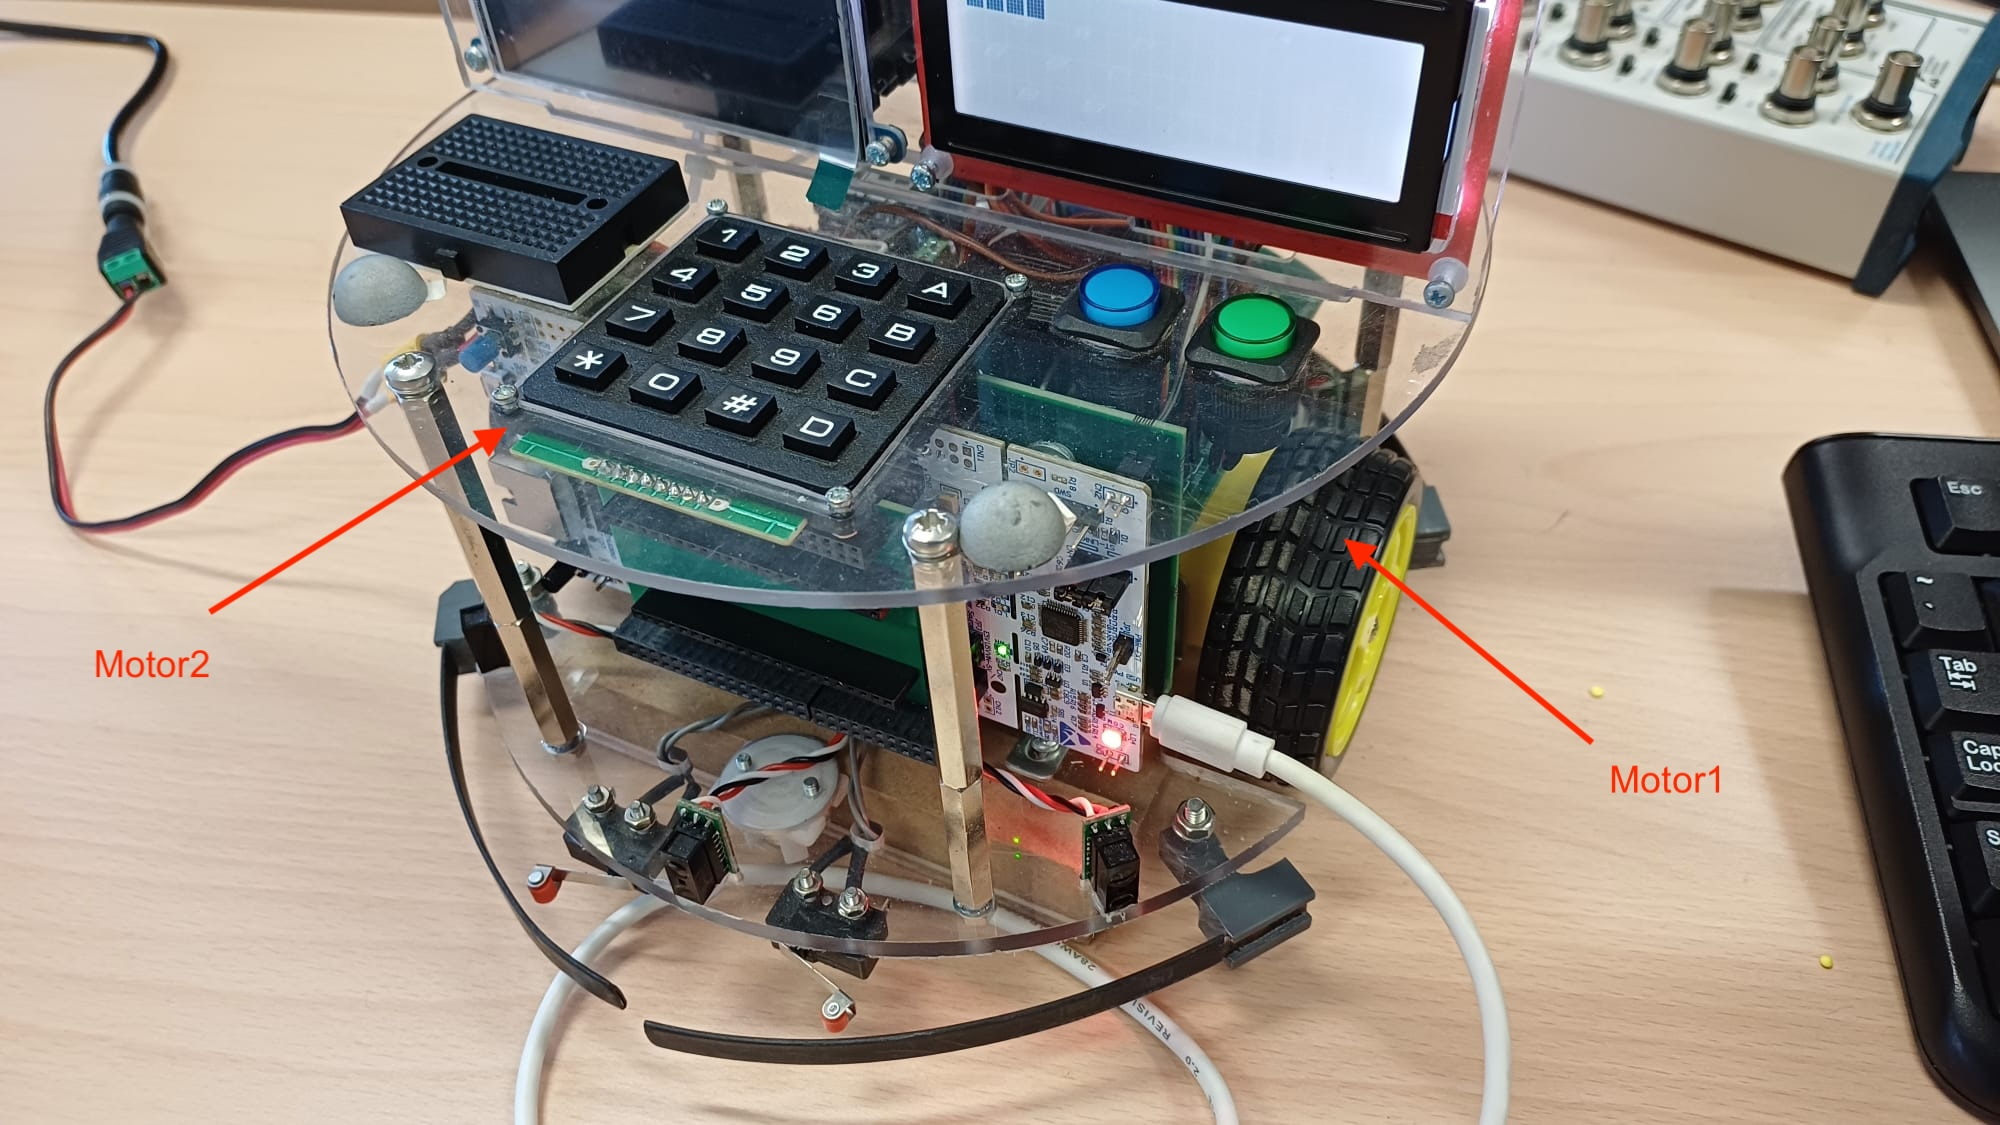
\includegraphics[width=0.55\textwidth]{figures/motor_id.jpeg}
  \caption{TurtleBot used in the experiment, with the position of motor~1 and motor~2.}
  \label{fig:lab2-setup}
\end{figure}

\begin{table}[H]
  \centering
  \small
  \begin{tabular}{@{}llll@{}}
    % tex-fmt: off
    \toprule
    File                                  & Drive mode & Direction                    & Used in                                     \\
    \midrule
    \texttt{motor\_data\_forward.mat}       & brake      & both forward                 & identification, controller design           \\
    \texttt{motor\_data\_reverse.mat}       & brake      & both reverse                 & direction comparison                        \\
    \texttt{motor\_data\_crossed.mat}       & brake      & motor~1 fwd, motor~2 rev     & check of the forward/reverse difference \\
    \texttt{motor\_data\_coast\_forward.mat} & coast      & both forward                 & drive-mode comparison                       \\
    \bottomrule
    % tex-fmt: on
  \end{tabular}
  \caption{Recorded data sets (each: five steps 2--6~V, $T_s=10$~ms, about 28~s).}
  \label{tab:lab2-datasets}
\end{table}

\paragraph{Choice of the step amplitudes.} We followed the first hypothesis of the lecture: no prior knowledge of the
operating point, so the parameters are estimated at several amplitudes and then compared. We used
$\{2,\,3,\,3.84,\,5,\,6\}$~V, which covers the whole range allowed by the 50\,\% limit. Both the 63.2\,\% method and
the tangent method were applied to all five steps; of the two, we kept the 63.2\,\% estimates because they are less
sensitive to noise on the derivative, as discussed in Section~\ref{sec:lab2-issues}. The reference voltage for the
controller design is $3.84$~V, that is $0.64\times6$~V: this value comes from the laboratory document and from the
lecture, where it is presented as the weighted operating point of the line-following task (the value $0.64$ itself is
a convention adopted in the course material).

\paragraph{Choice of the drive mode.} We used forward/brake (mode~2) for the identification, and we also recorded one
run in forward/coast (mode~3) to compare them (Section~\ref{sec:lab2-modes}). In brake mode the motor winding is
shorted during the off-time of the PWM, so the average voltage on the motor should be close to $D\cdot V_{batt}$ and
the speed should grow almost linearly with the voltage. In coast mode the bridge is open during the off-time and the
motor turns freely, so we expected a less linear behaviour. The coast data confirmed this: the gain and the time
constant change a lot with the step amplitude, while in brake mode they change much less. Since we want to describe
the motor with a single first-order model, brake mode is the better choice. Brake mode also stops the wheel at the
end of every step, and the current recirculates inside the bridge instead of going back to the bench power supply
through the body diodes.

\paragraph{Filtering.} The raw speed is affected by quantization and vibration, as visible in
Figure~\ref{fig:lab2-filter}. We filtered both signals with a first-order low-pass filter
\begin{equation}
  H(s) = \frac{2\pi f_c}{s+2\pi f_c}, \qquad f_c = 2~\text{Hz},
  \label{eq:lab2-filter}
\end{equation}
discretised with the Tustin method at $T_s=10$~ms. The cutoff frequency was chosen by comparing the filtered curve
with the raw data (Figure~\ref{fig:lab2-fc}): at 8~Hz the filter still passes too much noise, while at 0.8~Hz the
rise of the step is visibly delayed and the plateau is reached late. With $f_c=2$~Hz the quantization noise of the
plateau is removed and the rise keeps its shape. The price is a group delay of $1/(2\pi f_c)\approx0.08$~s; its
effect on the identified parameters is analysed in Section~\ref{sec:lab2-issues}.

\begin{figure}[H]
  \centering
  \subfloat[$f_c=0.8$~Hz]{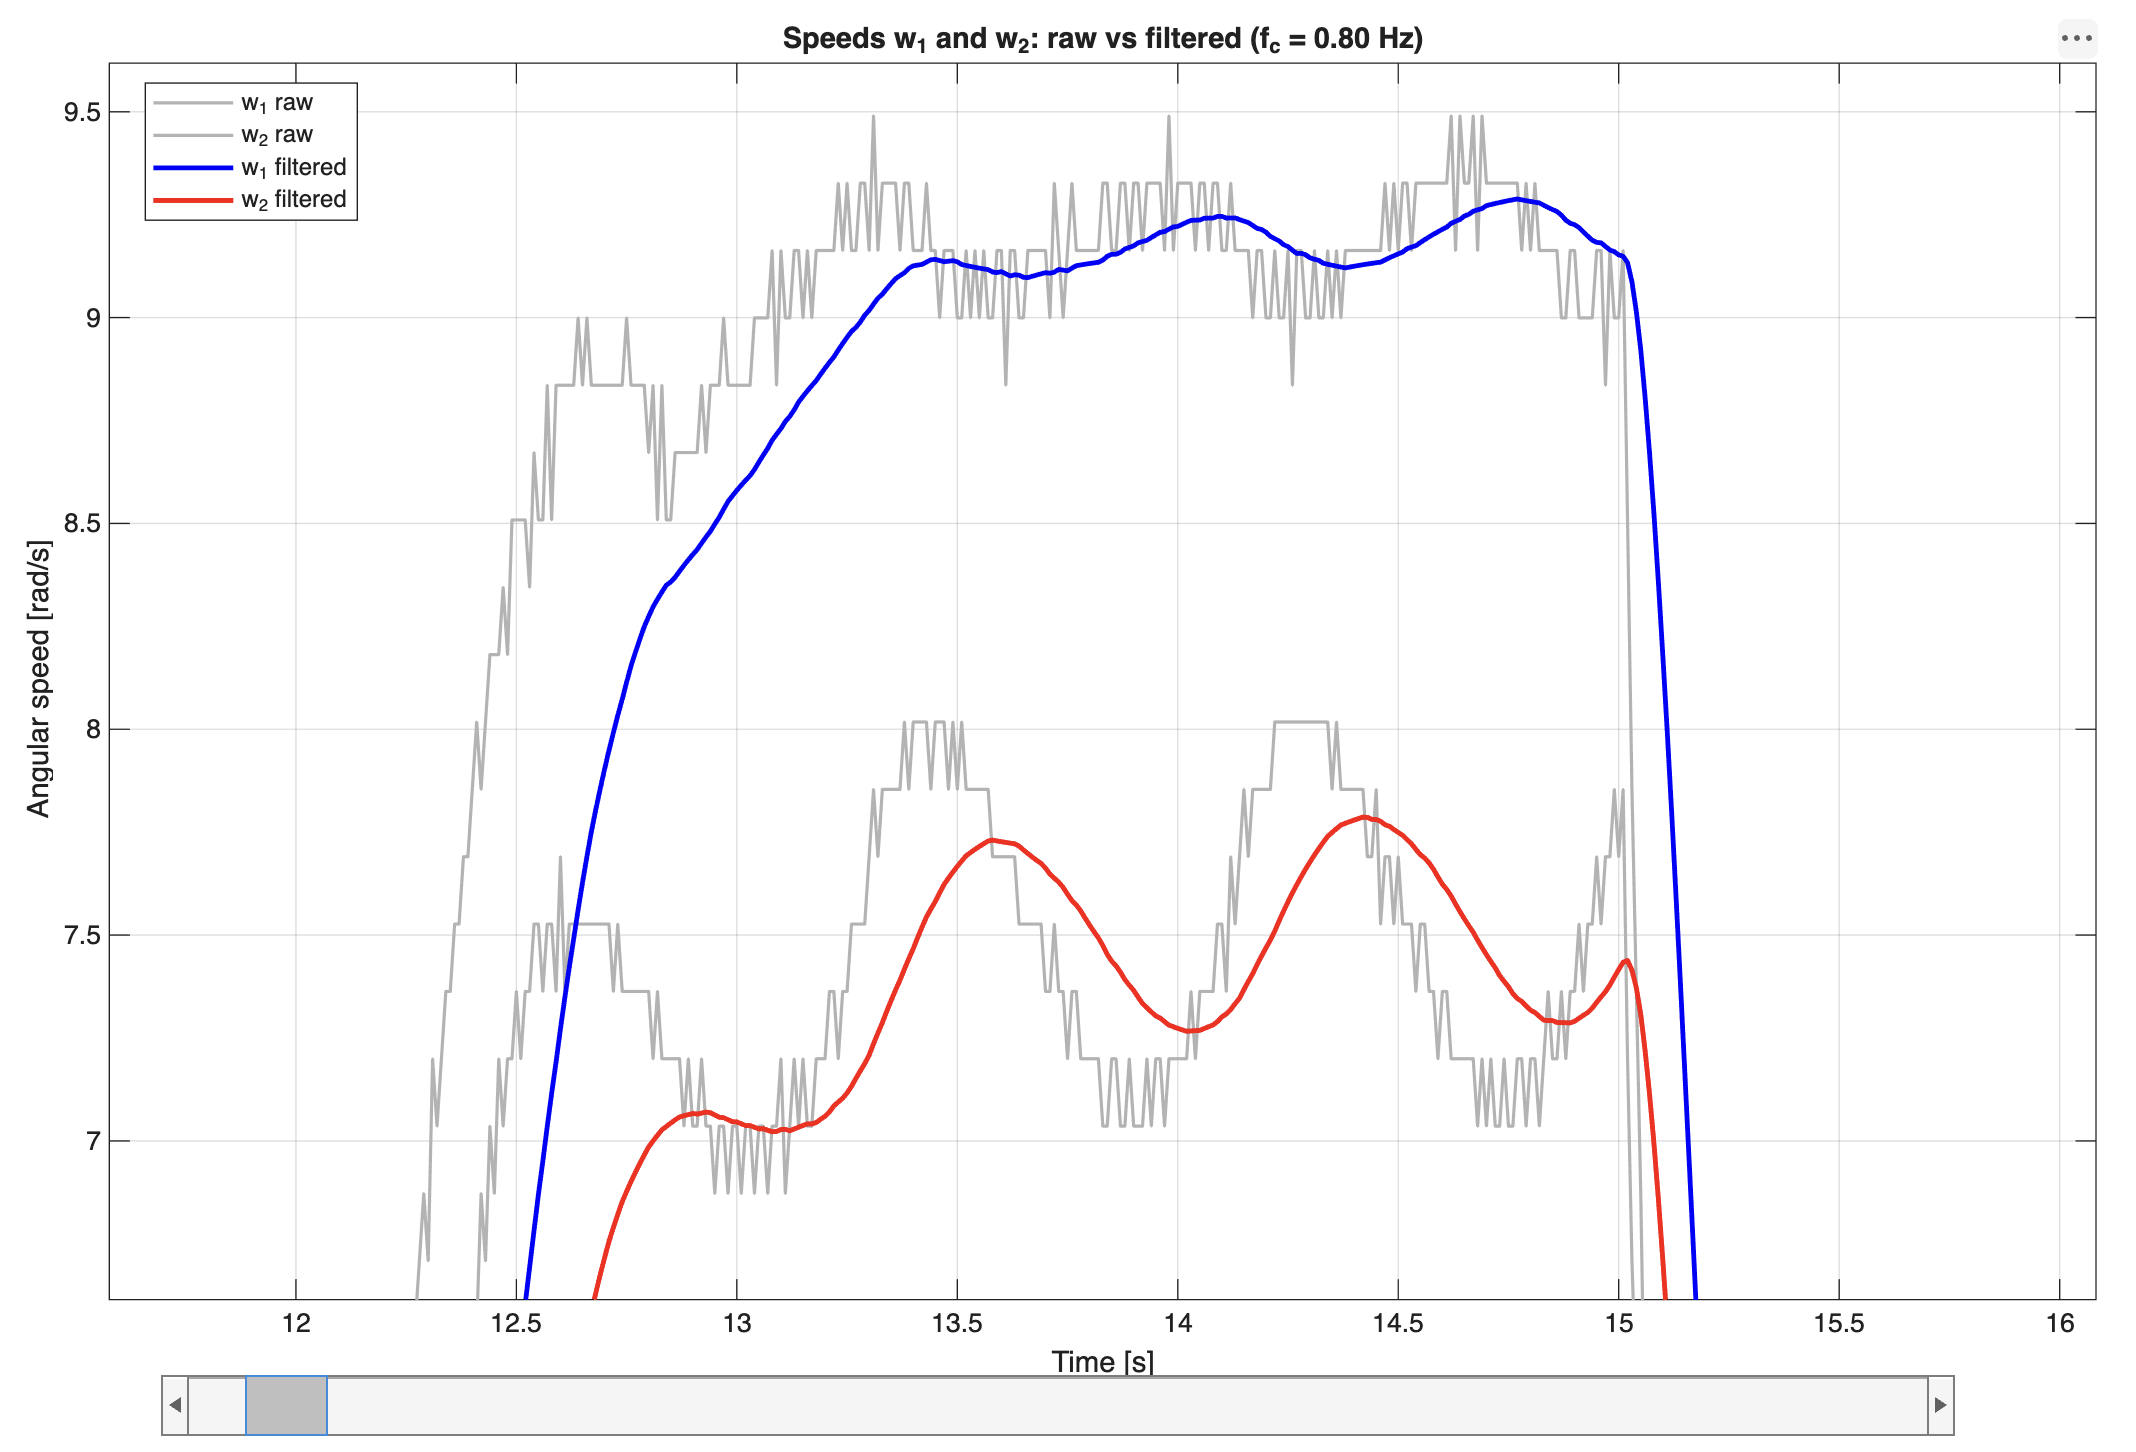
\includegraphics[width=0.32\textwidth]{figures/forward_underfit.png}}\hfill
  \subfloat[$f_c=2$~Hz (selected)]{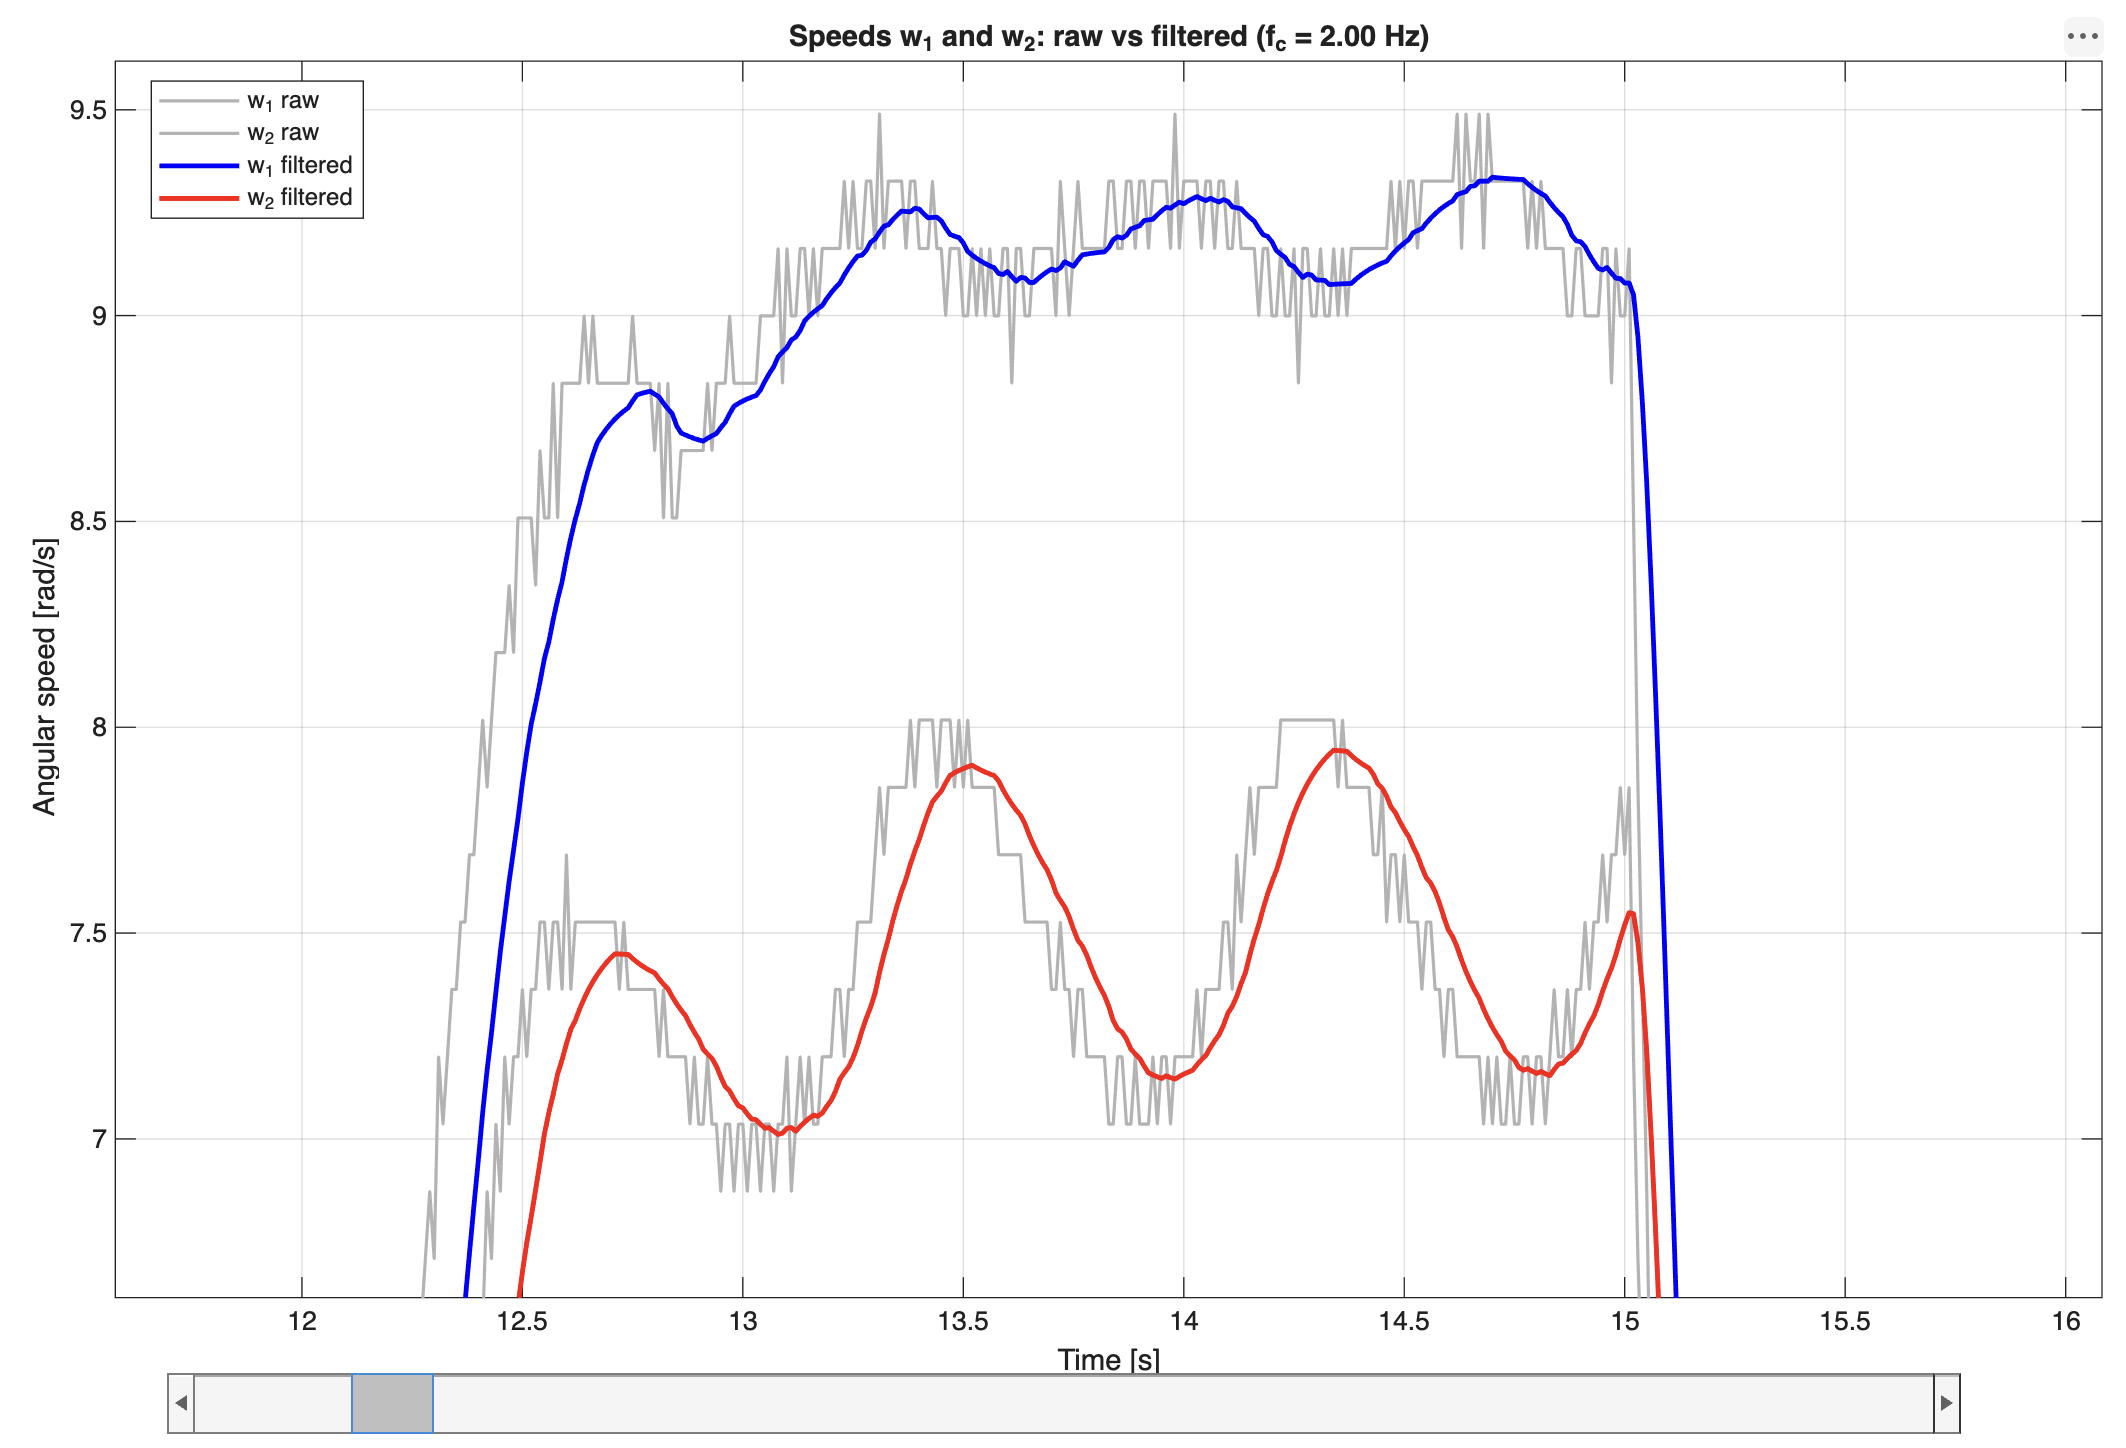
\includegraphics[width=0.32\textwidth]{figures/forward_selected.png}}\hfill
  \subfloat[$f_c=8$~Hz]{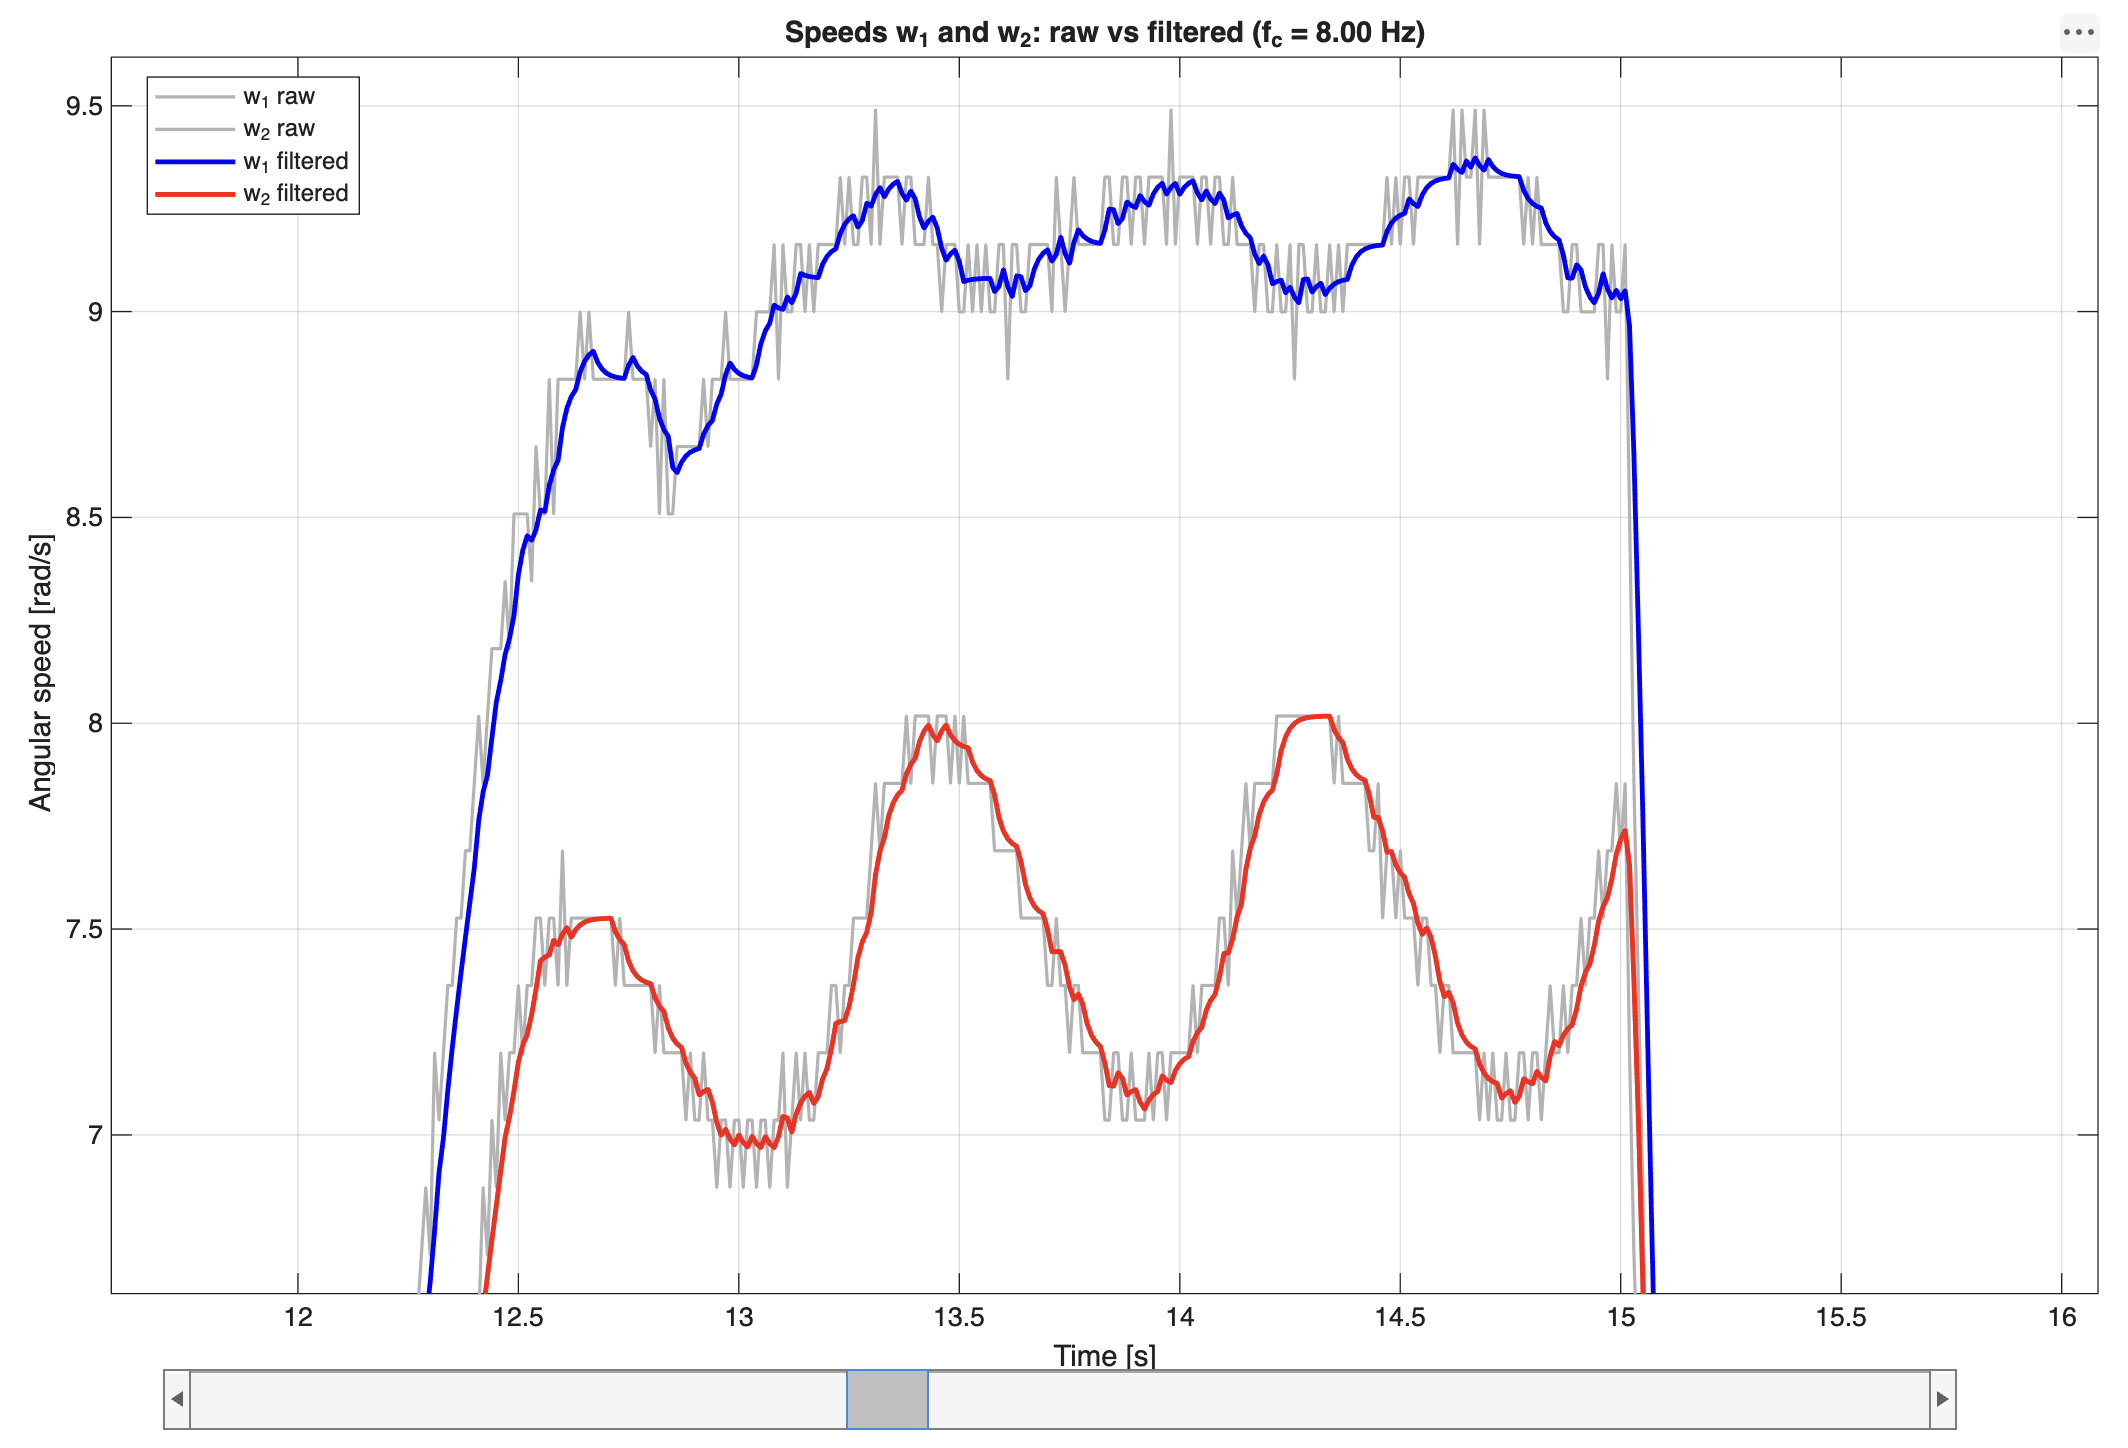
\includegraphics[width=0.32\textwidth]{figures/forward_overfit.png}}
  \caption{Choice of the filter cutoff on the 3.84~V step (grey: raw, blue: motor~1, red: motor~2).}
  \label{fig:lab2-fc}
\end{figure}

\paragraph{Data logging.} The firmware sends a packet of four floats (two speeds, two voltages) every 10~ms, encoded
with COBS and sent on USART3 at 115200 baud: 18 bytes take 1.6~ms, 16\,\% of the period. The time axis is not
transmitted: the MATLAB app adds $T_s=10$~ms per packet and the time vector assumes that no packet is lost. Both the
voltage and the speed are sent in the same packet because the PC and the TurtleBot are asynchronous systems: without
the voltage trace in the same acquisition it would be impossible to know exactly when the step was applied, and the
time constant and the delay could not be computed correctly.

\subsection{Controller Design}

\paragraph{Identified model.} The 63.2\,\% method applied to the step at 3.84~V gives, for motor~1,
$\mu=2.408$~rad/s/V, $T=0.26$~s and $\tau=0.06$~s; for motor~2 it gives $\mu=1.916$~rad/s/V, $T=0.25$~s and the same
delay. The two motors are not identical, and the gain differs by about 20\,\%. Most of this delay actually comes
from the filter (Section~\ref{sec:lab2-issues}), but we kept this model for the design, for the reasons explained
there.

\paragraph{Ziegler--Nichols.} Both identification methods were applied to all five steps; the open-loop Ziegler--Nichols
rules \eqref{eq:lab2-zn} were then evaluated on the 63.2\,\% estimates at $V_a=3.84$~V. For motor~1 this gives
$K_p=1.620$ and $K_i=8.998$ ($T_i=0.18$~s). As a cross-check we also computed the closed-loop variant of the method
on the identified model: the critical frequency is the solution of $-\omega\tau-\arctan(\omega T)=-\pi$, which gives
$\omega_c=28.4$~rad/s, $T_{cr}=0.221$~s and $K_{cr}=3.10$; the PI row of the table then gives $K_p=1.394$,
$T_i=0.184$~s and $K_i=7.56$. The two sets are close, a good consistency check; the open-loop method was chosen
because it uses only the measured step response. The same procedure applied to motor~2 ($\mu=1.916$, $T=0.25$~s,
$\tau=0.06$~s) gives the second pair of gains stored in the firmware; the closed-loop variant gives $K_{cr}=3.76$ and
$T_{cr}=0.220$~s. Table~\ref{tab:lab2-gains} summarises the values.

\paragraph{Why Ziegler--Nichols.} We wanted a speed loop that is faster than the open-loop motor
($T\approx0.25$~s) and has no steady-state error. We chose Ziegler--Nichols because it only needs the three parameters
we had already identified, without any other experiment, and because it was presented in the lectures. We also know
that this method gives quite aggressive gains, so we checked the stability margins and the effect of the 6~V
saturation in simulation (Section~\ref{sec:lab2-results}).

\begin{table}[H]
  \centering
  \small
  \begin{tabular}{@{}llccc@{}}
    % tex-fmt: off
    \toprule
    Motor & Method                            & $K_p$  & $T_i$ [s] & $K_i$   \\
    \midrule
    1     & Ziegler--Nichols open loop (used) & 1.6196 & 0.180     & 8.9979  \\
    1     & Ziegler--Nichols closed loop      & 1.3935 & 0.184     & 7.5644  \\
    2     & Ziegler--Nichols open loop (used) & 1.9574 & 0.180     & 10.8747 \\
    2     & Ziegler--Nichols closed loop      & 1.6900 & 0.184     & 9.2001  \\
    \bottomrule
    % tex-fmt: on
  \end{tabular}
  \caption{PI gains obtained from the identified models. The rows marked ``used'' are the constants
    \texttt{KP1/KI1} and \texttt{KP2/KI2} of the firmware.}
  \label{tab:lab2-gains}
\end{table}

\noindent The proportional gain is larger for motor~2 only because its static gain is smaller: the product
$K_p\mu$ is similar for the two wheels, so the two loops have a comparable bandwidth. The controller is implemented
as a discrete PI with forward Euler integration, exactly as in the lecture:
\begin{equation}
  u(k) = K_p\,e(k) + I(k), \qquad I(k) = I(k-1) + K_i\,T_s\,e(k) .
  \label{eq:lab2-pi}
\end{equation}
A separate PI instance is kept for each wheel (separate proportional and integral gains, separate integral state),
because the integral term must persist across calls and must not be shared between the two motors.

\subsection{Discovered Issues, Calibration \& Workarounds}
\label{sec:lab2-issues}

\paragraph{Delay introduced by the filter.} When we first tried the identification on the raw signal, the
derivative had spikes of about 70~rad/s$^2$ (Figure~\ref{fig:lab2-deriv}) and the tangent was completely wrong.
Filtering solved this problem but moved the start of the response to the right. With the 63.2\,\% method we found
$\tau\approx0.05$--$0.06$~s on all five steps, which is very close to the group delay of the filter (0.08~s), so we
suspected that most of this delay was not real. To check it, we analysed the 3.84~V step again in three ways that do
not add any delay: the 63.2\,\% method on the signal filtered with \texttt{filtfilt} (the same filter applied
forward and then backward, so that the delays cancel), the 63.2\,\% method on the raw signal, and a least-squares fit
of the first-order model on the raw signal. The results are in Table~\ref{tab:lab2-delay} and
Figure~\ref{fig:lab2-delay}.

\begin{table}[H]
  \centering
  \small
  \begin{tabular}{@{}lcccccc@{}}
    % tex-fmt: off
    \toprule
                                          & \multicolumn{3}{c}{Motor 1} & \multicolumn{3}{c}{Motor 2} \\
    \cmidrule(lr){2-4}\cmidrule(lr){5-7}
    Method                                & $\mu$ [rad/s/V] & $T$ [s] & $\tau$ [s] & $\mu$ [rad/s/V] & $T$ [s] & $\tau$ [s] \\
    \midrule
    63.2\,\%, causal LPF (design model)   & 2.408 & 0.26  & 0.06  & 1.916 & 0.25  & 0.06  \\
    Tangent, causal LPF                   & 2.408 & 0.377 & 0.048 & 1.916 & 0.372 & 0.043 \\
    63.2\,\%, zero-phase LPF              & 2.342 & 0.24  & 0.00  & 1.864 & 0.23  & 0.00  \\
    63.2\,\%, raw signal                  & 2.404 & 0.19  & 0.03  & 1.906 & 0.20  & 0.02  \\
    Least-squares fit, raw signal         & 2.387 & 0.206 & 0.011 & 1.950 & 0.191 & 0.016 \\
    \bottomrule
    % tex-fmt: on
  \end{tabular}
  \caption{Parameters of the 3.84~V step obtained with and without the delay of the filter.}
  \label{tab:lab2-delay}
\end{table}

\begin{figure}[H]
  \centering
  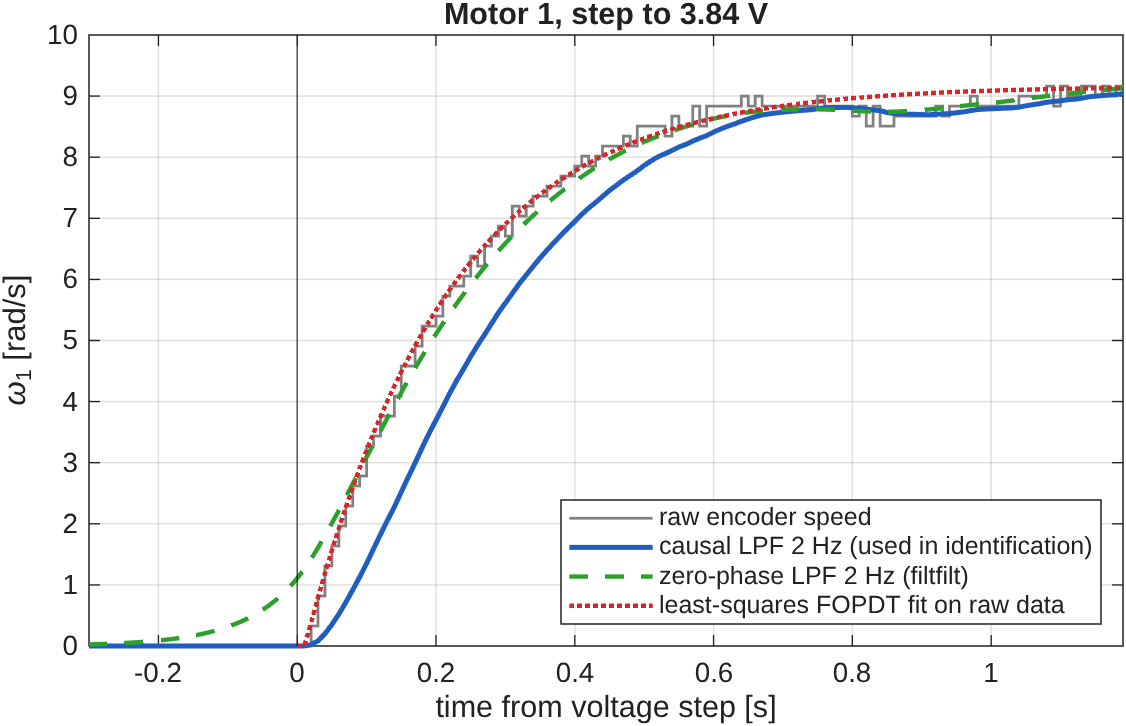
\includegraphics[width=0.70\textwidth]{figures/filter_delay.png}
  \caption{The 3.84~V step of motor~1: raw speed, causal and zero-phase filtered speed, and the least-squares
    first-order fit. The causal filter shifts the response by about 0.05--0.08~s.}
  \label{fig:lab2-delay}
\end{figure}

\noindent The three methods without delay give similar results: the delay is about one sample (0.01--0.02~s), which
makes sense because each speed sample is an average over the previous 10~ms, and the time constant is between 0.19
and 0.24~s instead of 0.26~s. The gain is almost the same in all cases. The \texttt{filtfilt} result is not useful
for the delay: since it also uses future samples, the filtered response starts slightly before the step (green curve
in Figure~\ref{fig:lab2-delay}), so it always gives $\tau=0$. In the end we decided to keep the model obtained with
the causal filter for the controller design. Ziegler--Nichols needs a delay greater than zero, and with
$\tau\approx0.01$~s it would give $K_p\approx7$, which would saturate the 6~V output for almost any step. Using a
model with more delay than the real motor should give less aggressive gains, and in Section~\ref{sec:lab2-results}
we verified this on the fitted model.

\begin{figure}[H]
  \centering
  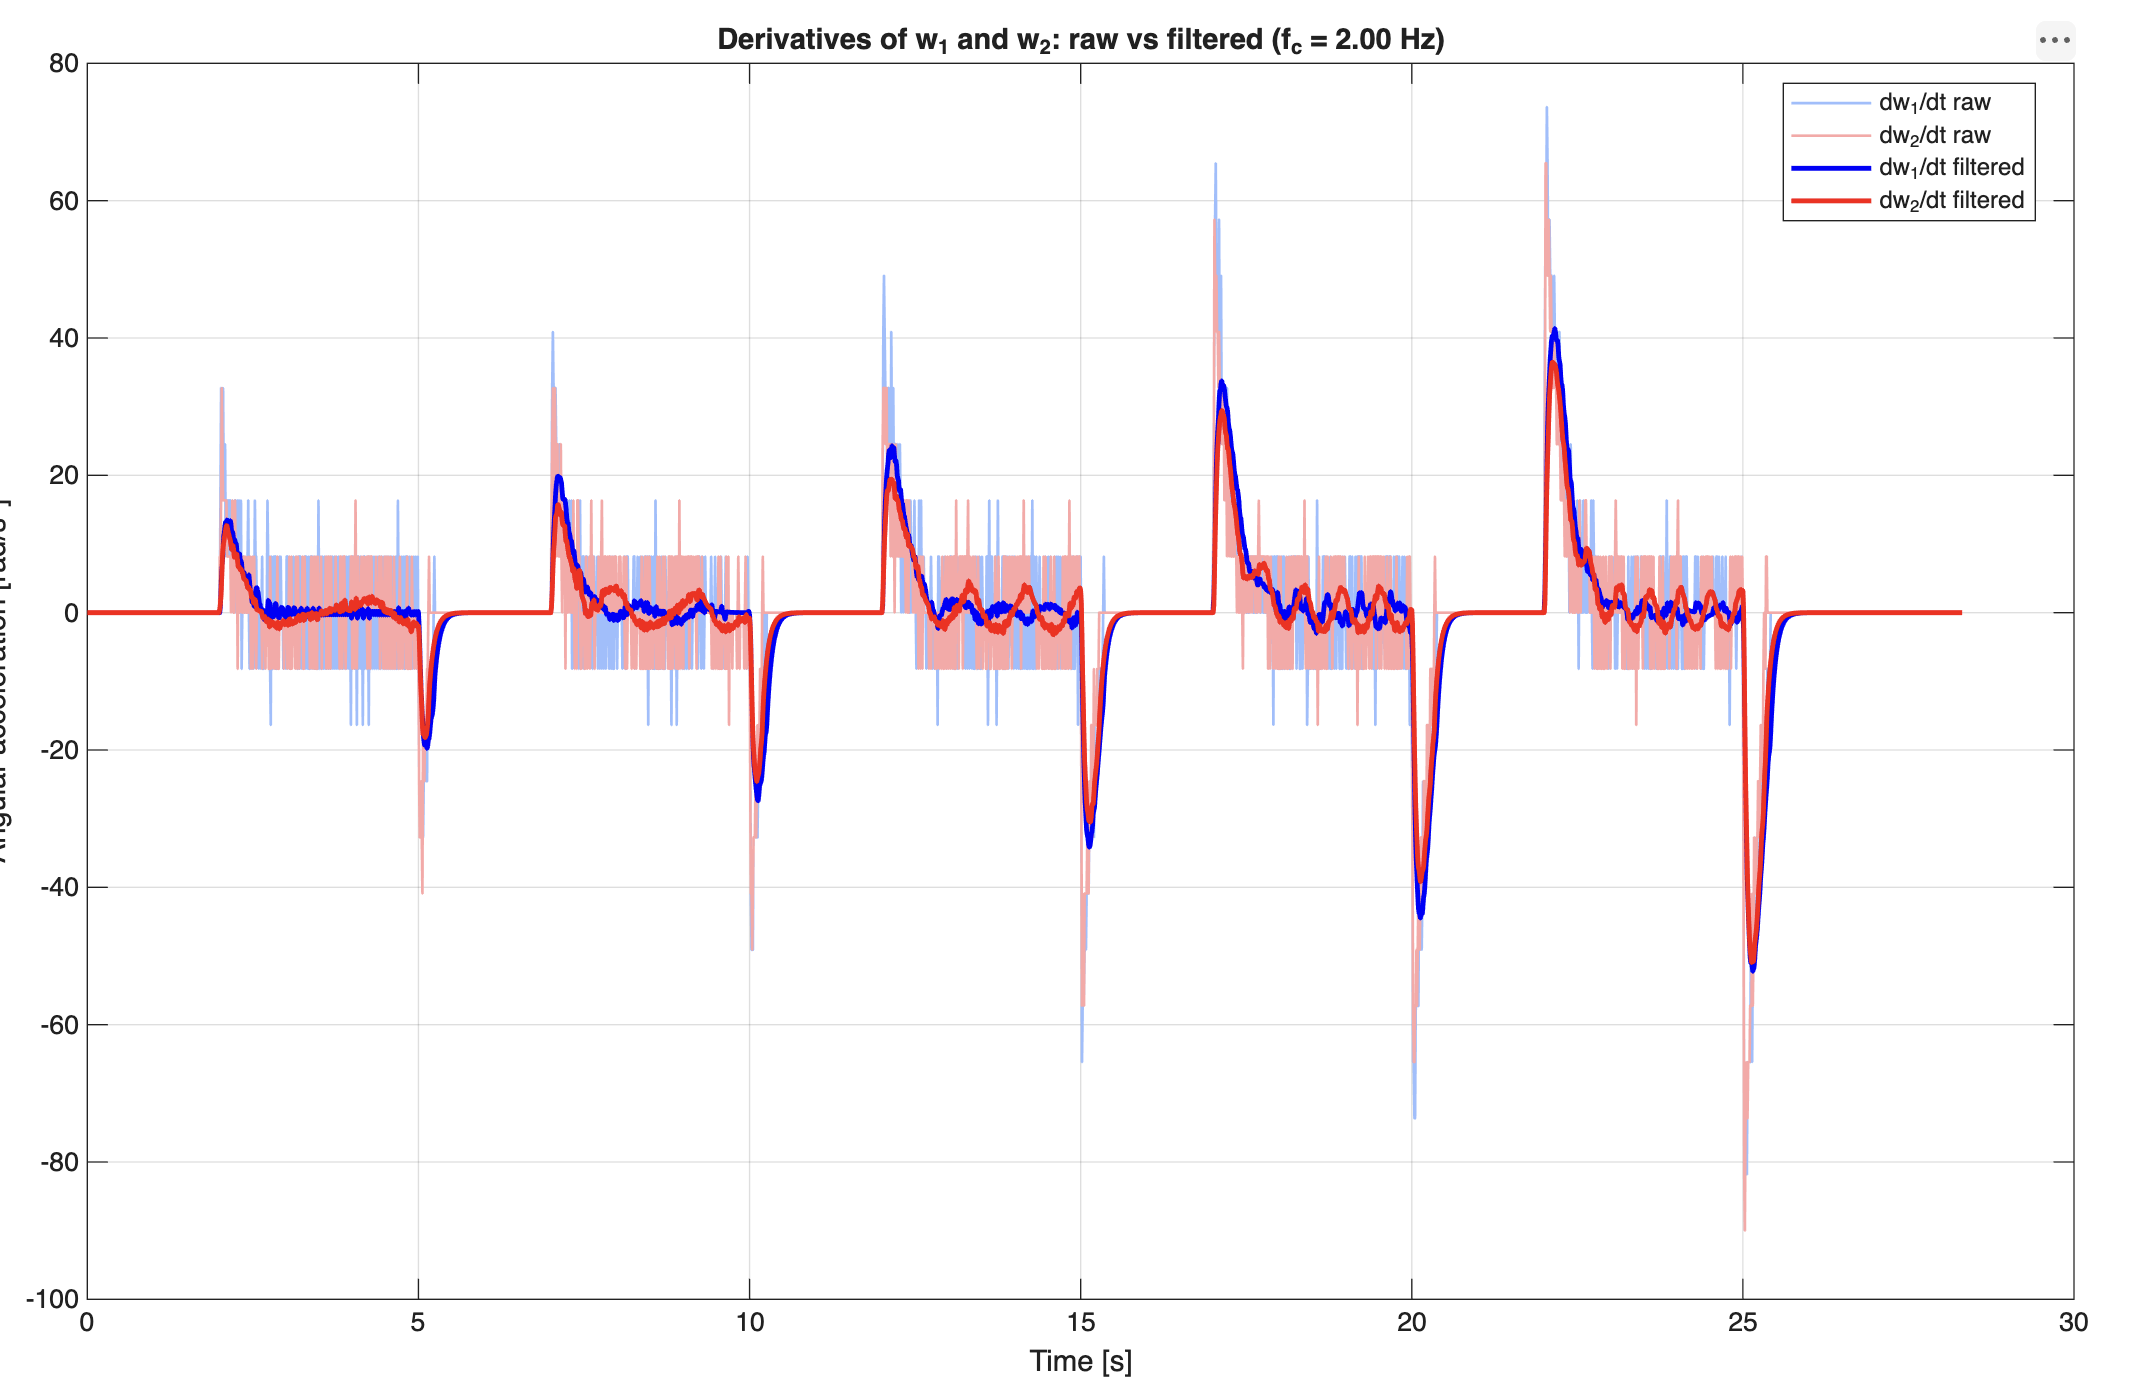
\includegraphics[width=0.70\textwidth]{figures/speed_derivates.png}
  \caption{Derivative of the raw and filtered speeds over the whole sequence. The raw derivative is dominated by
    the quantization of the encoder (one count in 10~ms is 16~rad/s$^2$ of derivative).}
  \label{fig:lab2-deriv}
\end{figure}

\paragraph{Tangent method versus 63.2\,\% method.} Both methods were applied to all five steps of both motors
(Tables~\ref{tab:lab2-identification} and~\ref{tab:lab2-identification-m2}, Figure~\ref{fig:lab2-tangent}). The
tangent method gives $T\approx0.27$--$0.40$~s, about 45\,\% larger than the 63.2\,\% method on the same filtered
signal, and nearly twice the value of the least-squares fit on the raw data. The reason is that the filter reduces
the maximum slope, and a smaller slope in \eqref{eq:lab2-tangent} gives a larger $T$. The tangent method is therefore
correct in principle but biased by the filtering, and for this reason we used the 63.2\,\%
estimates for the controller.
\begin{figure}[H]
  \centering
  \subfloat[Motor 1]{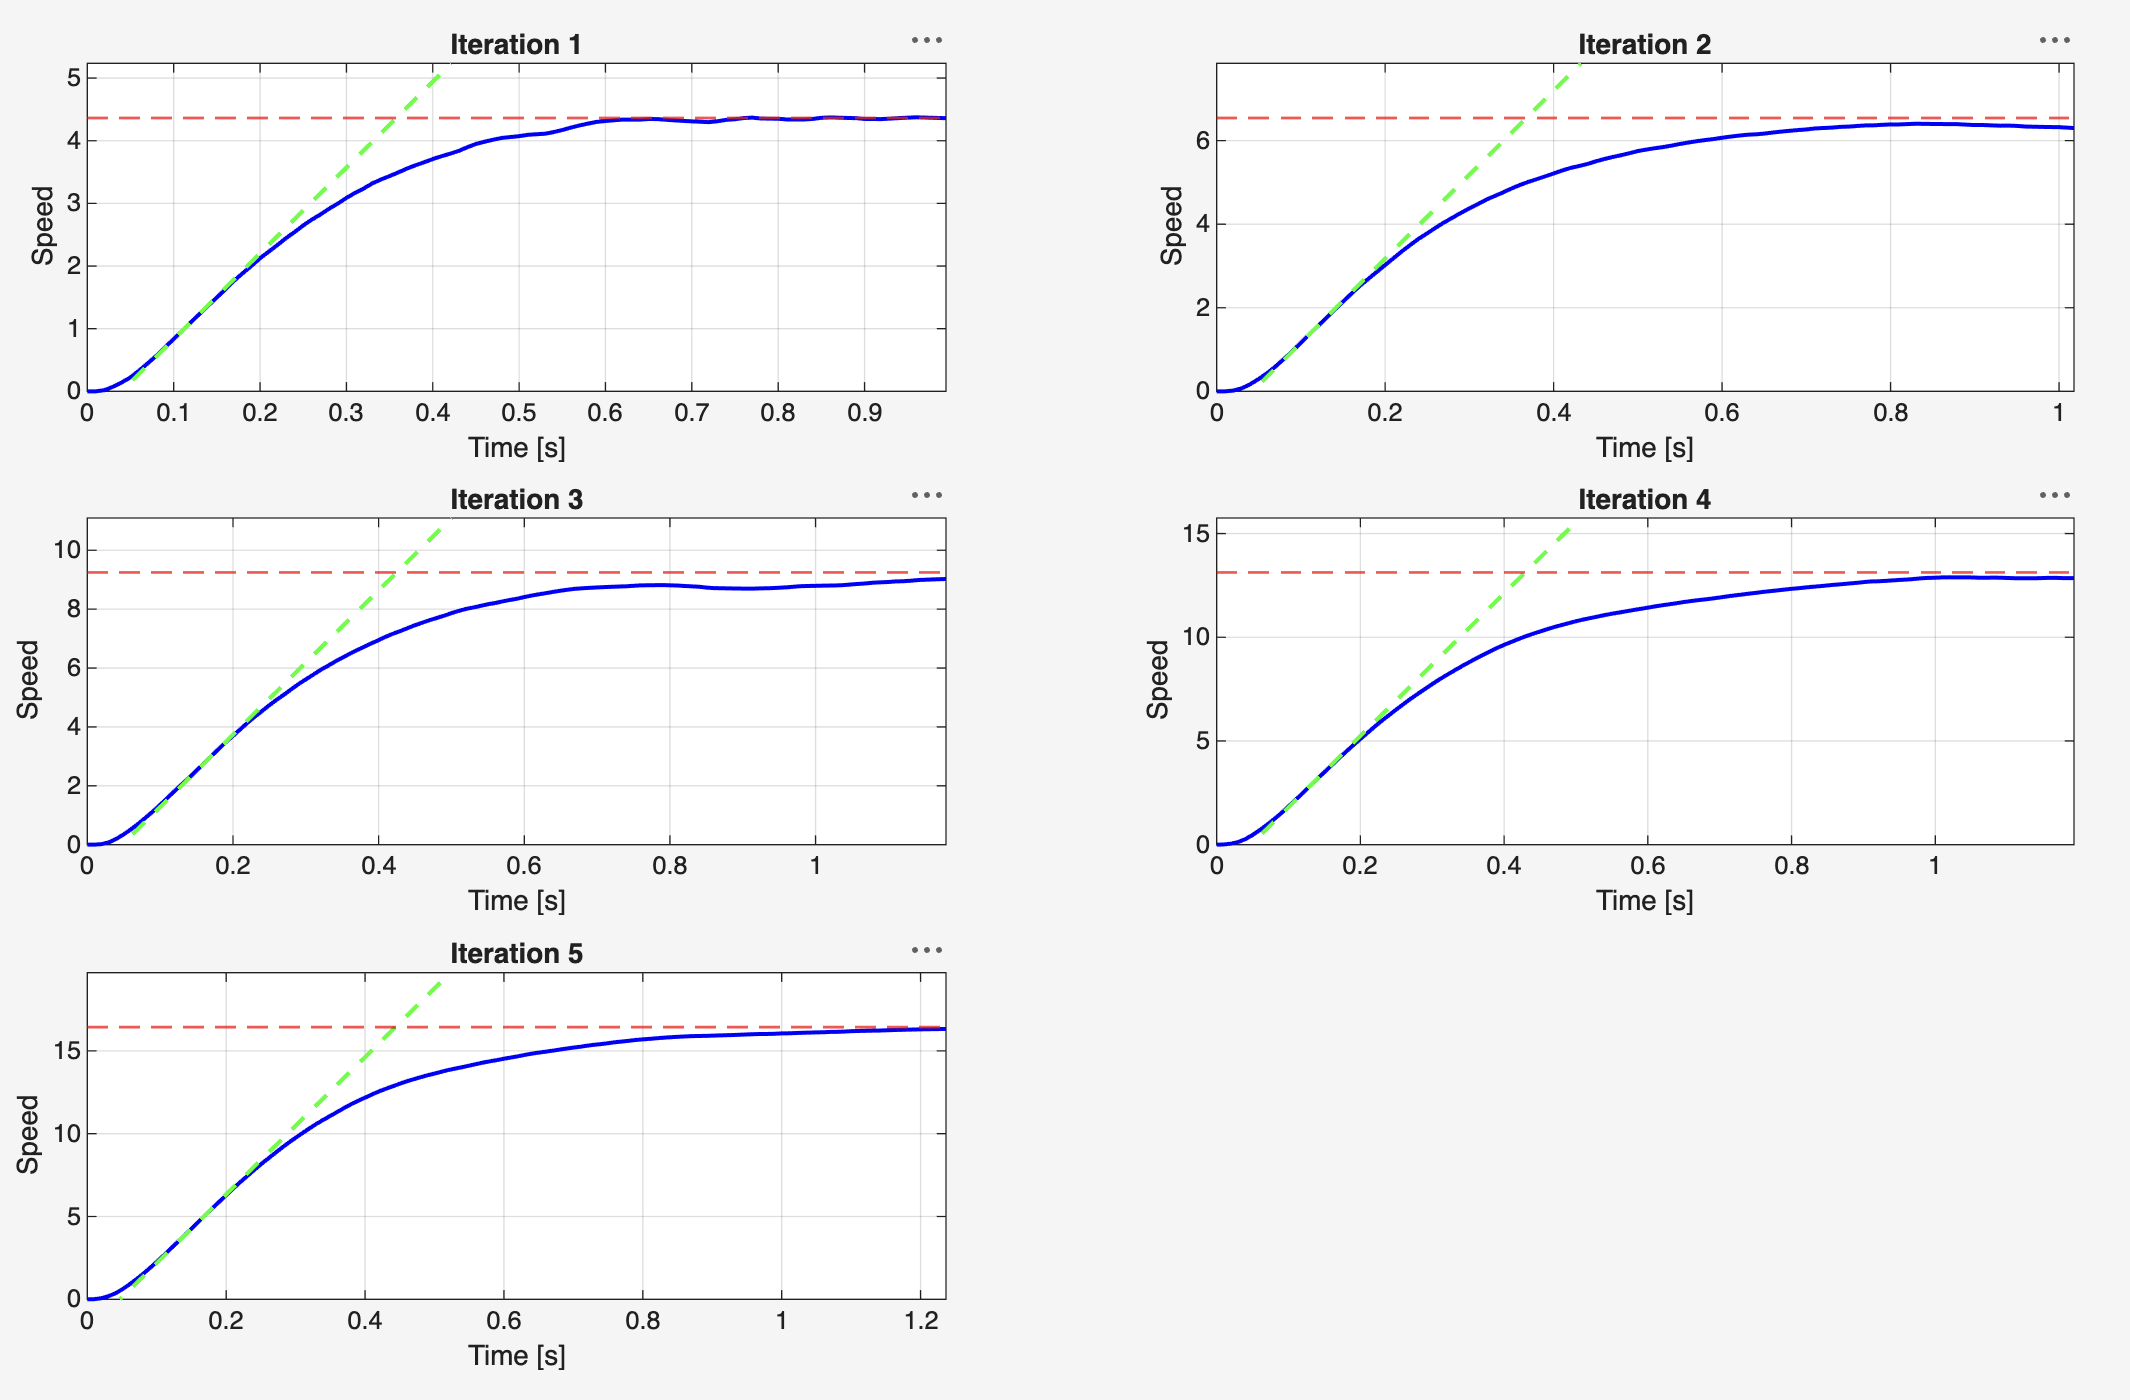
\includegraphics[width=0.48\textwidth]{tangent/tangent_graph_m1.png}}\hfill
  \subfloat[Motor 2]{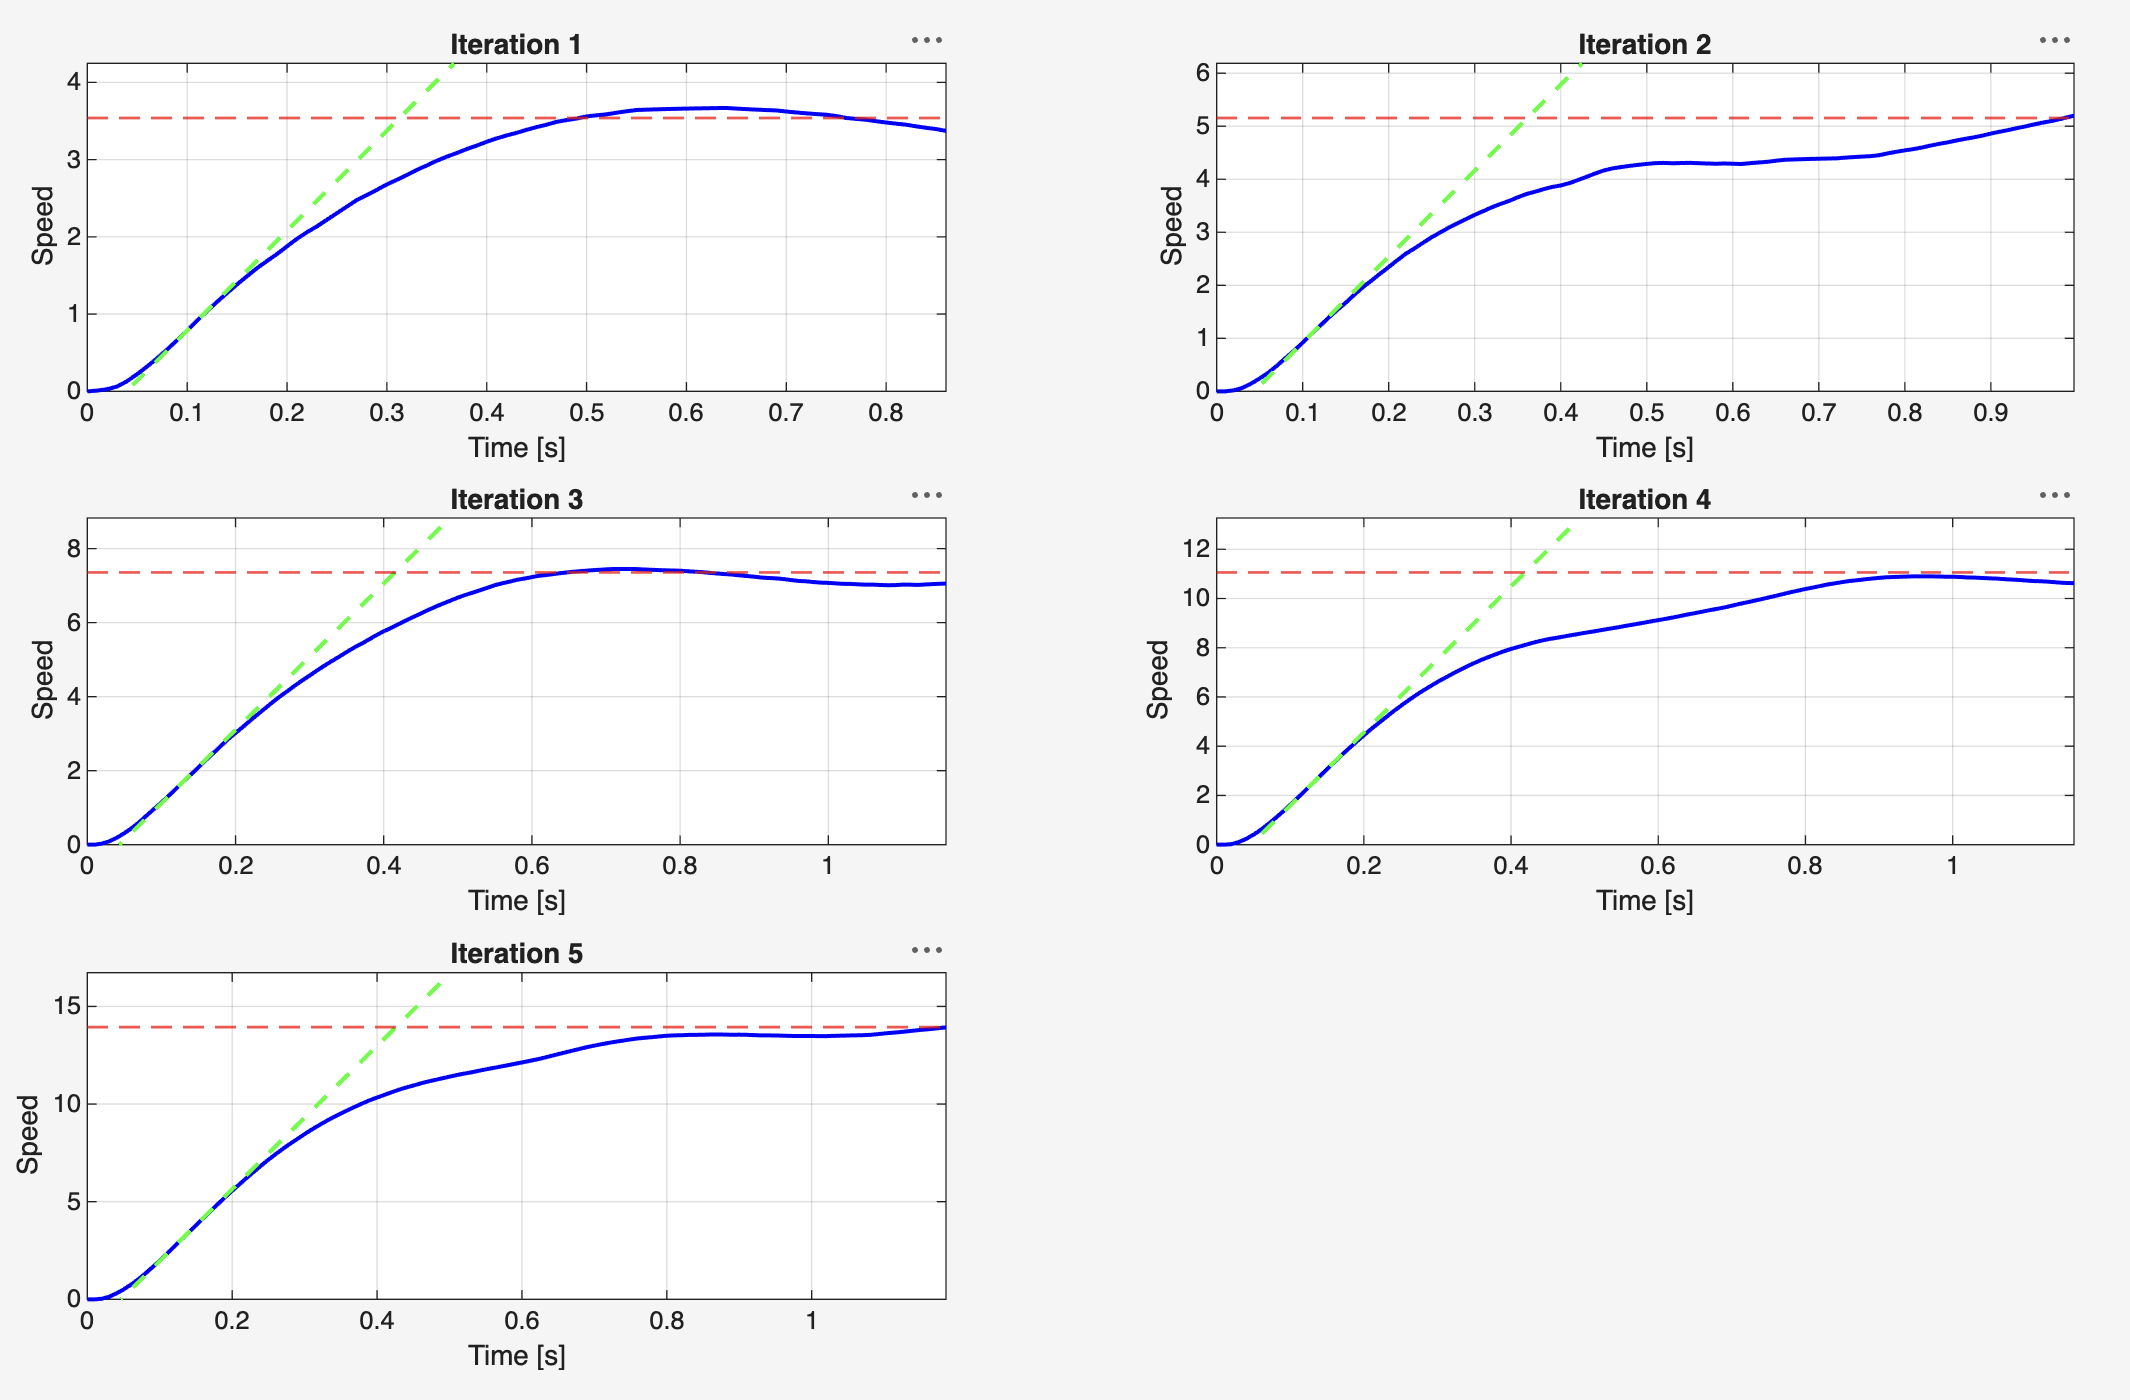
\includegraphics[width=0.48\textwidth]{tangent/tangent_graph_m2.png}}
  \caption{Tangent method on the five filtered steps: response (blue), tangent at the point of maximum slope (green)
    and steady-state level (red).}
  \label{fig:lab2-tangent}
\end{figure}

\paragraph{Non-linearity of the motor.} The estimated gain is not constant: for motor~1 it grows from
2.18~rad/s/V at 2~V to 2.74~rad/s/V at 6~V (+25\,\%), and the time constant from 0.22 to 0.27~s; motor~2 shows the
same overall trend (from 1.77 at 2~V to 2.32~rad/s/V at 6~V). We think that at low voltage the friction takes a larger part of the torque, so
the speed per volt is lower. This is why the lecture suggests several operating points; since the gain
varies with the voltage, the controller is designed at the chosen reference point $V_a=3.84$~V.


\paragraph{Supply voltage.} The firmware declares \texttt{VBATT = 12}~V, which matches the bench power supply used
in the laboratory. The motor is rated for about 6~V, so the duty cycle is limited to 50\,\% to apply at most 6~V
to the motor.

\paragraph{Integral wind-up in the simulation.} The first closed-loop simulation used the PI of \eqref{eq:lab2-pi}
with a simple saturation of the output. For motor~1 and a 10~rad/s reference, during the initial transient the
controller asks for more than 6~V, the output stays at 6~V for 0.68~s, but the integral keeps accumulating. The
result is a peak of 13.5~rad/s, that is a 35\,\% overshoot, with a settling time of 1.2~s. Re-running the same
simulation with conditional integration (the integral is updated only when the output is not saturated or when the
error pushes it back) reduces the overshoot to 0.1\,\% and the settling time to 0.6~s. For motor~2 the overshoot is
smaller but the problem is still there: 10~rad/s needs 5.2~V in steady state, which is very close to the limit, so
the output stays saturated for 1.8~s and the settling time becomes 2.3~s; with anti-windup it is 0.7~s. The firmware
will need the same correction in Laboratory~3, and the speed reference should stay well below the maximum speed of
each motor.

\paragraph{Time axis and lost packets.} A dropped packet does not create a gap, so the recording simply becomes
shorter. With the blocking UART transmission inside the interrupt the margin is only 8.4~ms per period, so the packet
rate is the first thing to check when the identification looks inconsistent.

\subsection{Results and Graphical Analysis}
\label{sec:lab2-results}

Figure~\ref{fig:lab2-filter} shows the five-step experiment after filtering. The two wheels reach different speeds,
as expected from the different gains, and the response of motor~1 is cleaner. The plateaus are flat, which confirms
that three seconds are enough to reach the steady state (more than ten time constants); motor~2 shows a small
oscillation on the plateau, whose frequency matches the rotation frequency of the wheel, so it is probably caused by
the wheel or the gearbox (for example a slight eccentricity).
\begin{figure}[H]
  \centering
  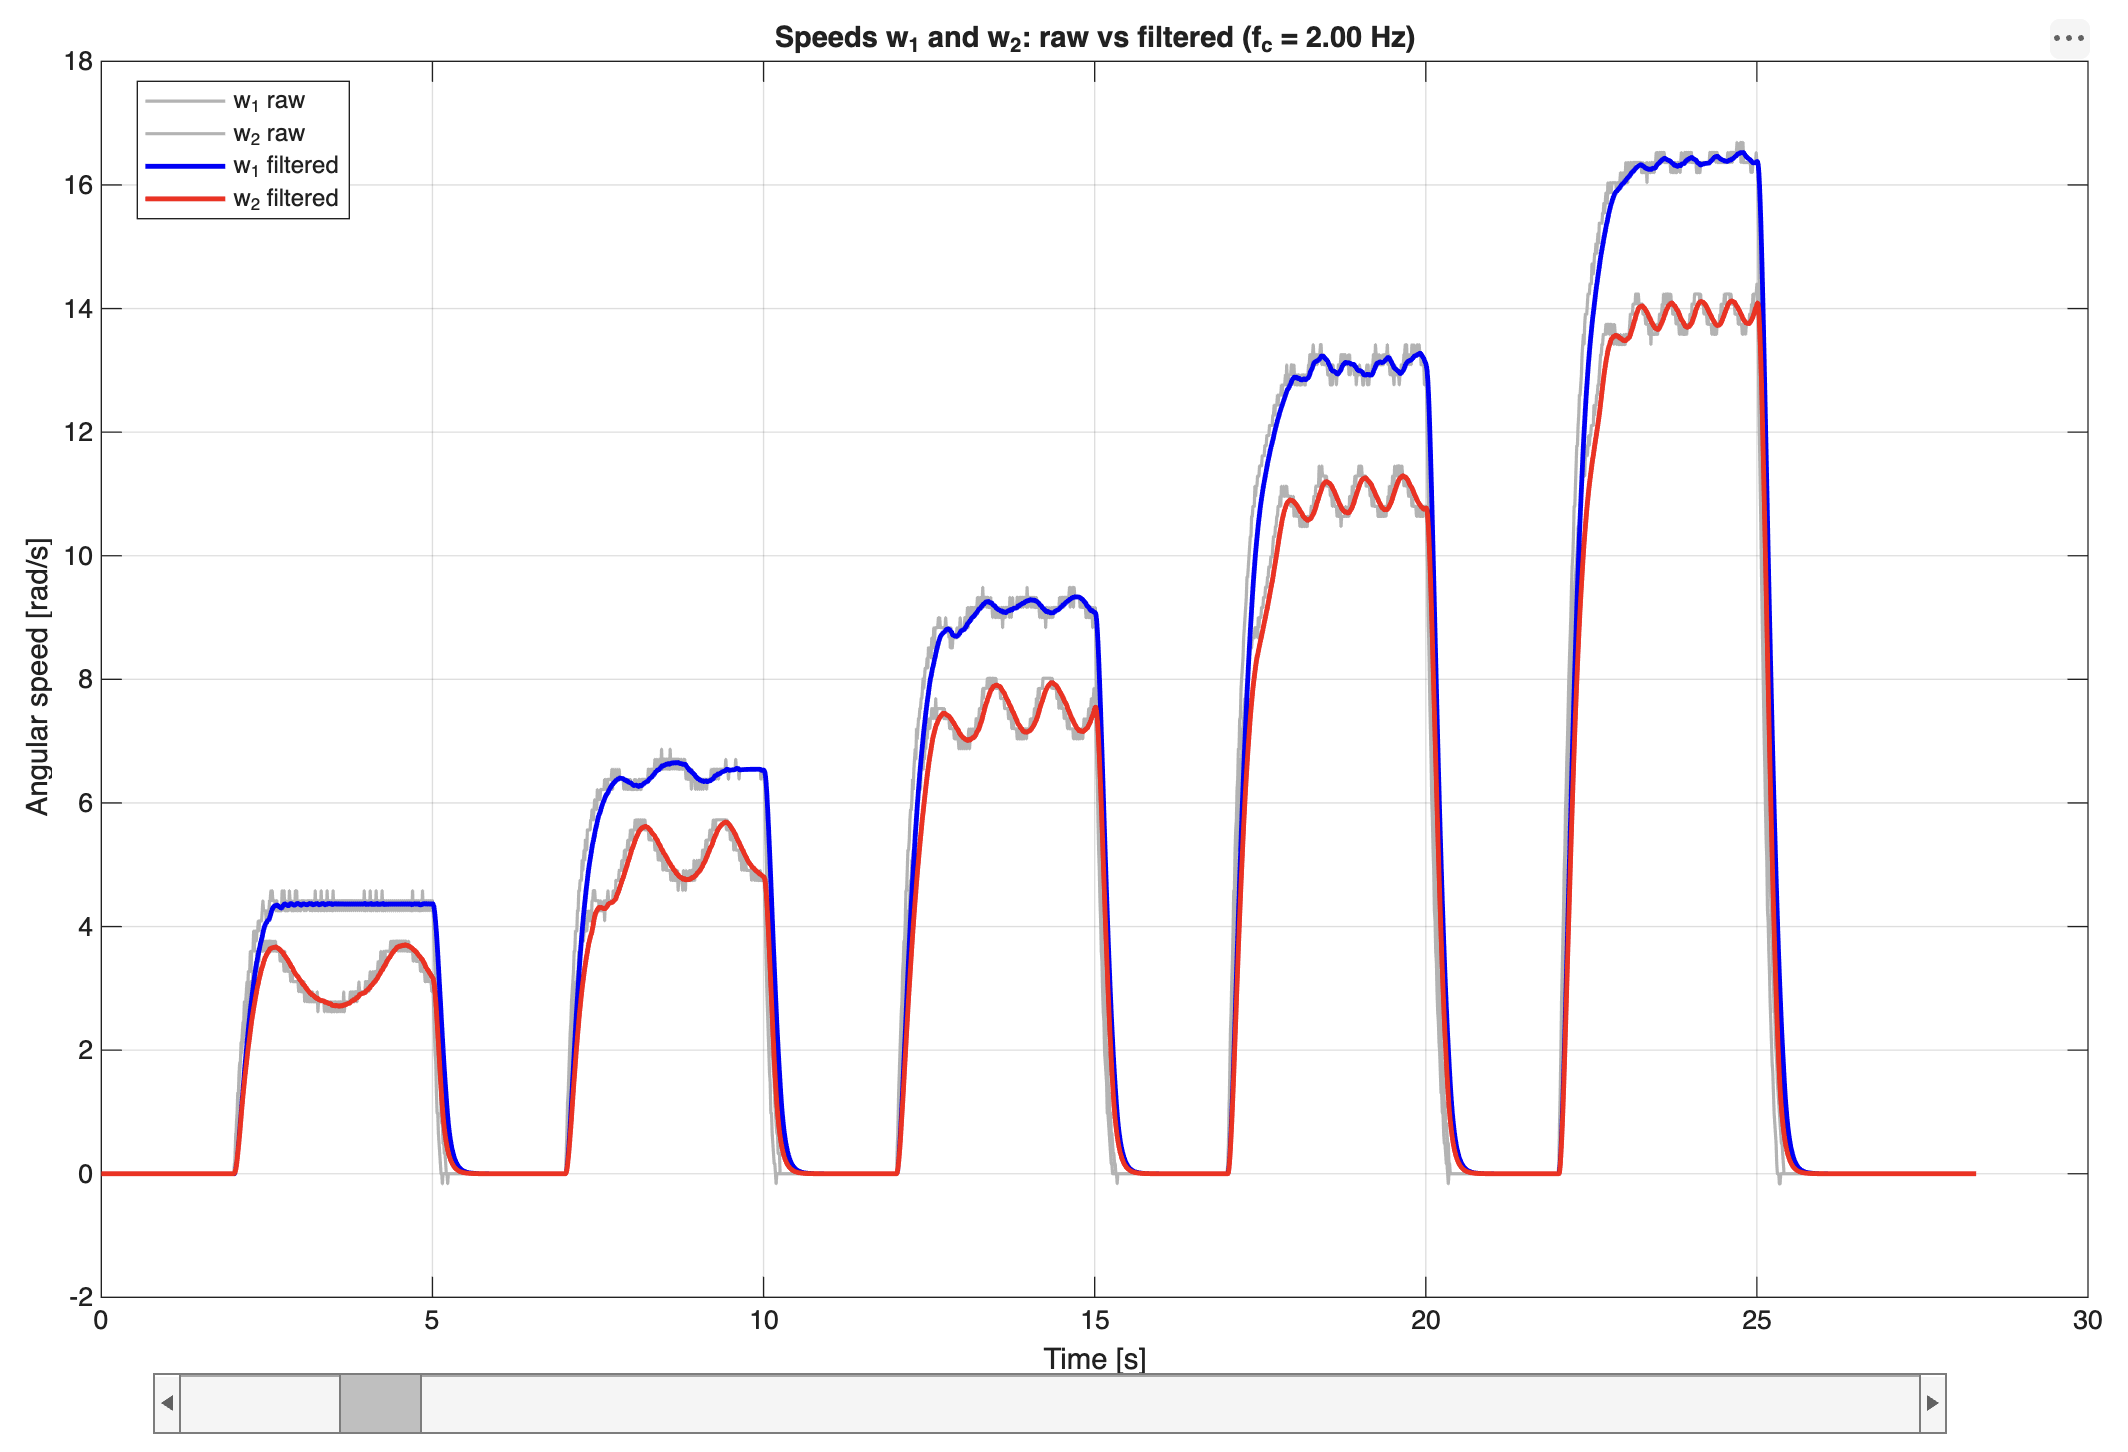
\includegraphics[width=0.70\textwidth]{figures/filtered_all.png}
  \caption{Measured speeds of the two wheels, raw and filtered with $f_c=2$~Hz, during the five-step sequence.}
  \label{fig:lab2-filter}
\end{figure}

\noindent Table~\ref{tab:lab2-identification} collects the estimates of motor~1 for the five amplitudes, obtained with
the two methods. The gain increases with the amplitude, while the delay is essentially constant; the 63.2\,\% method
gives the same time constant for the last two steps, which suggests that the motor is close to saturation there.

\begin{table}[H]
  \centering
  \small
  \begin{tabular}{@{}cccccccc@{}}
    % tex-fmt: off
    \toprule
    Step   & $V_a$ [V] & $f_\infty$ [rad/s] & $\mu$ [rad/s/V] & $T_{63}$ [s] & $\tau_{63}$ [s] & $T_{tan}$ [s] & $\tau_{tan}$ [s] \\
    \midrule
    1      & 2.00      & 4.36               & 2.181           & 0.22         & 0.050           & 0.318         & 0.039            \\
    2      & 3.00      & 6.54               & 2.180           & 0.22         & 0.060           & 0.325         & 0.042            \\
    3      & 3.84      & 9.25               & 2.408           & 0.26         & 0.060           & 0.377         & 0.048            \\
    4      & 5.00      & 13.12              & 2.625           & 0.27         & 0.060           & 0.382         & 0.048            \\
    5      & 6.00      & 16.43              & 2.739           & 0.27         & 0.060           & 0.397         & 0.047            \\
    \midrule
    mean   & --        & --                 & 2.427           & 0.248        & 0.058           & 0.360         & 0.045            \\
    median & --        & --                 & 2.408           & 0.260        & 0.060           & 0.377         & 0.048            \\
    \bottomrule
    % tex-fmt: on
  \end{tabular}
  \caption{Identification of motor~1 with the 63.2\,\% method and with the tangent method.}
  \label{tab:lab2-identification}
\end{table}

\noindent Table~\ref{tab:lab2-identification-m2} gives the same analysis for motor~2. The behaviour is the same as for
motor~1, with a gain about 20\,\% lower at every amplitude and very similar time constants and delays, so the two
motors differ mainly in their static gain.

\begin{table}[H]
  \centering
  \small
  \begin{tabular}{@{}cccccccc@{}}
    % tex-fmt: off
    \toprule
    Step   & $V_a$ [V] & $f_\infty$ [rad/s] & $\mu$ [rad/s/V] & $T_{63}$ [s] & $\tau_{63}$ [s] & $T_{tan}$ [s] & $\tau_{tan}$ [s] \\
    \midrule
    1      & 2.00      & 3.54               & 1.769           & 0.20         & 0.050           & 0.274         & 0.039            \\
    2      & 3.00      & 5.16               & 1.718           & 0.24         & 0.060           & 0.318         & 0.043            \\
    3      & 3.84      & 7.36               & 1.916           & 0.25         & 0.060           & 0.372         & 0.043            \\
    4      & 5.00      & 11.06              & 2.212           & 0.27         & 0.060           & 0.373         & 0.046            \\
    5      & 6.00      & 13.94              & 2.324           & 0.26         & 0.060           & 0.380         & 0.046            \\
    \midrule
    mean   & --        & --                 & 1.988           & 0.244        & 0.058           & 0.343         & 0.044            \\
    median & --        & --                 & 1.916           & 0.250        & 0.060           & 0.372         & 0.043            \\
    \bottomrule
    % tex-fmt: on
  \end{tabular}
  \caption{Identification of motor~2 with the 63.2\,\% method and with the tangent method.}
  \label{tab:lab2-identification-m2}
\end{table}

\noindent Figure~\ref{fig:lab2-openloop} compares the measured speed with the two theoretical models, $G(s)$ without
delay and $P(s)=\mu e^{-\tau s}/(1+Ts)$, driven by the recorded voltage. The model follows the five transients well,
and the difference between $G$ and $P$ is small, which confirms that the delay is not the dominant term. The
steady-state speed is slightly overestimated at 2~V and 3~V because a single linear gain cannot reproduce the
friction at low speed. This is the expected effect of the non-linearity described above and it is the reason why the
model is used near its operating point.

\begin{figure}[H]
  \centering
  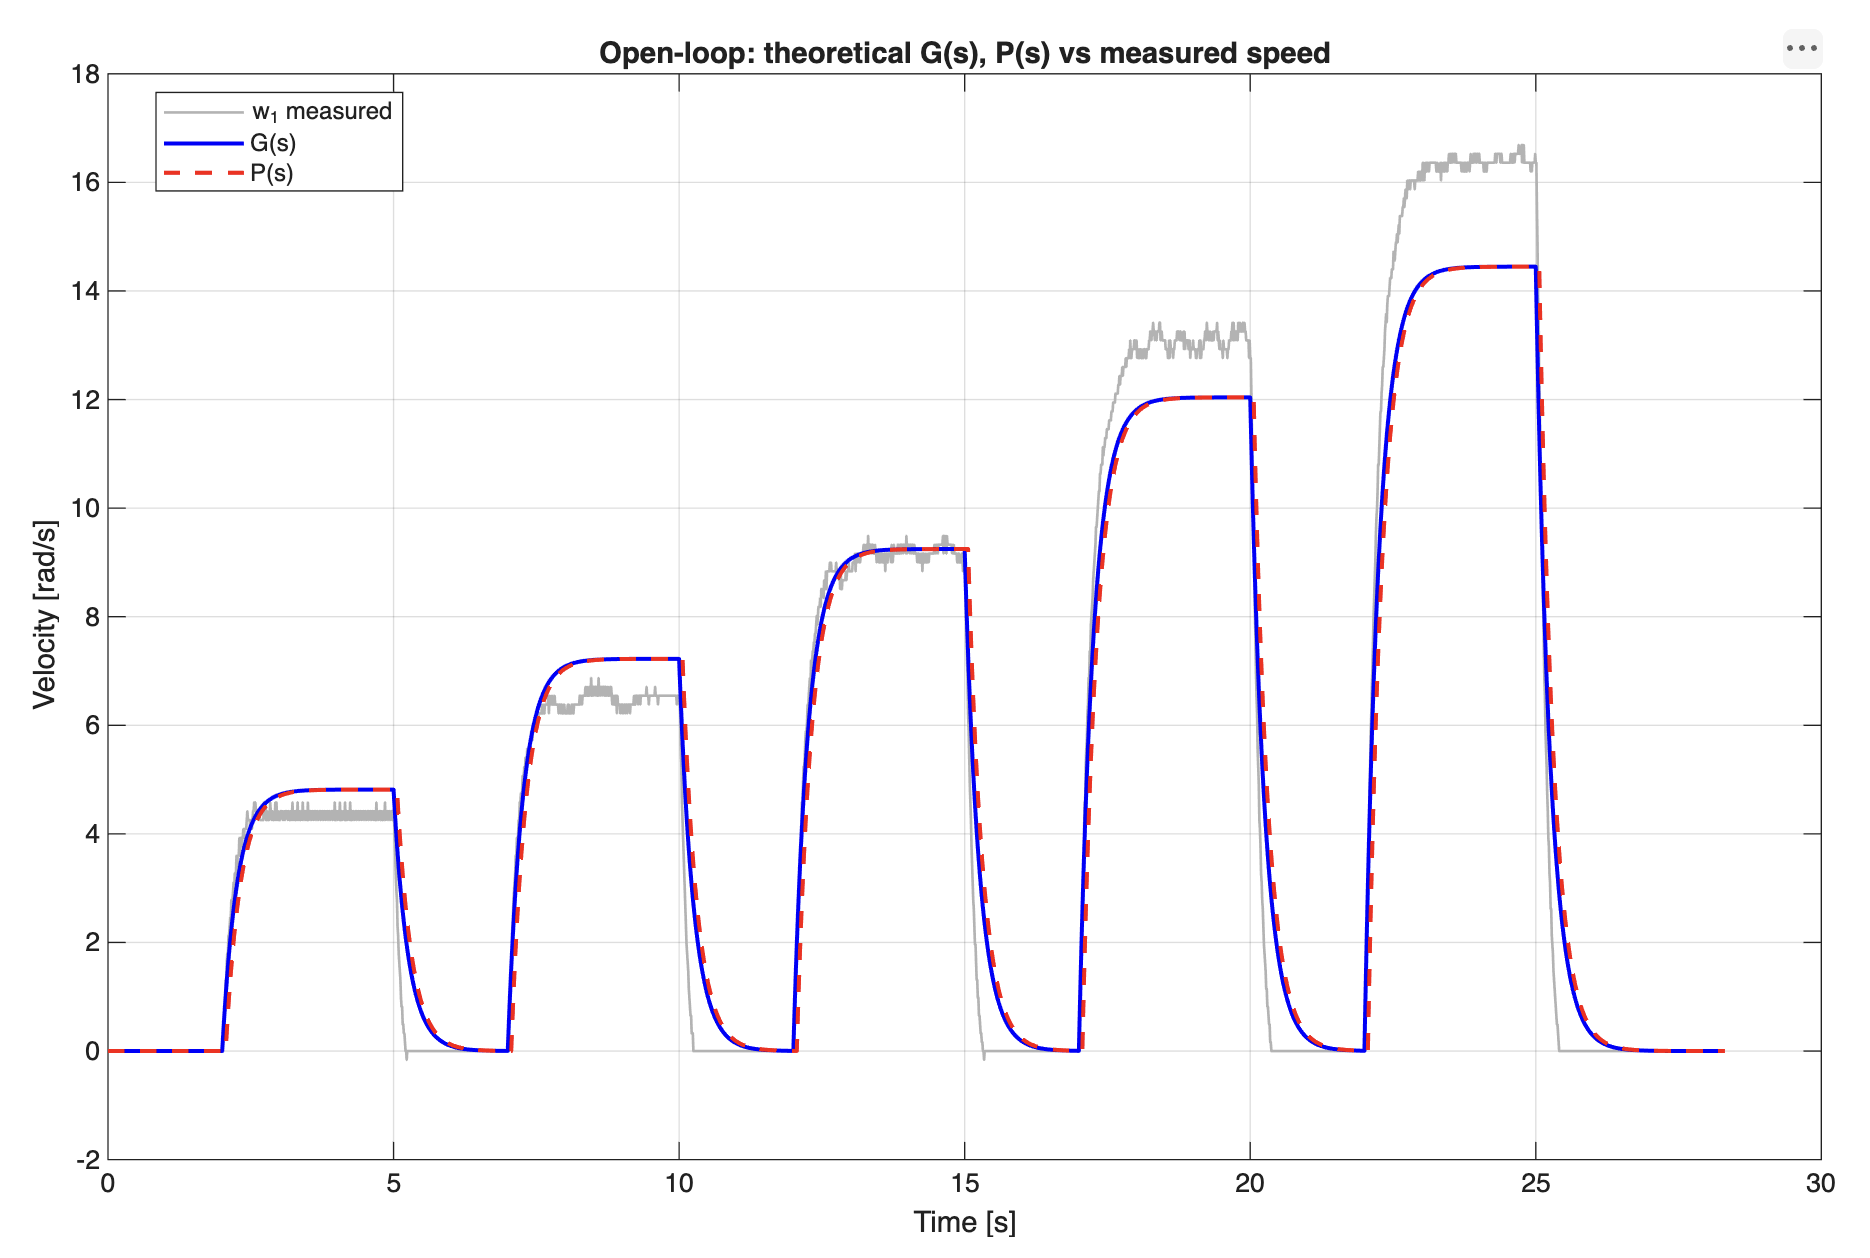
\includegraphics[width=0.70\textwidth]{figures/open-loop_simulation.png}
  \caption{Open-loop validation: measured speed of motor~1 compared with $G(s)$ and $P(s)$ driven by the recorded
    voltage.}
  \label{fig:lab2-openloop}
\end{figure}

\subsubsection{Drive modes and direction of rotation}
\label{sec:lab2-modes}

We applied the same identification (63.2\,\% method, same filter) to the coast and reverse recordings.
Figure~\ref{fig:lab2-modes} shows the gain and the time constant as a function of the step amplitude for all cases,
and Table~\ref{tab:lab2-modes} gives the values at the operating point.

\begin{figure}[H]
  \centering
  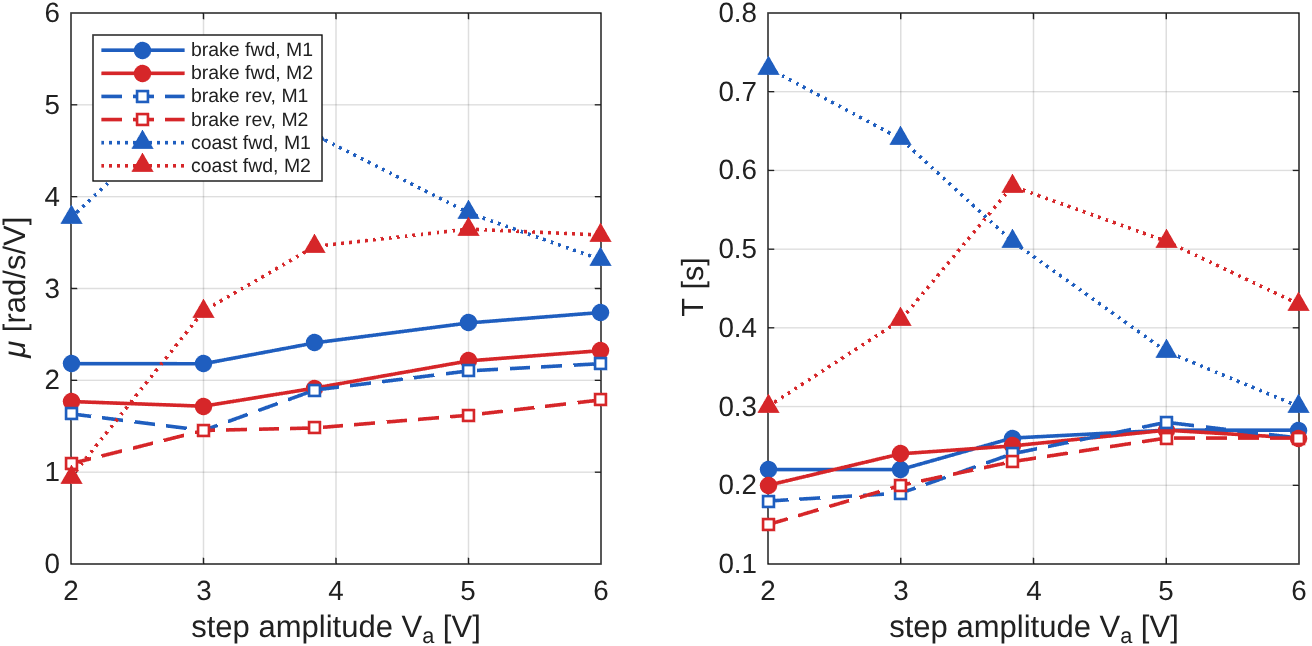
\includegraphics[width=0.85\textwidth]{figures/params_vs_voltage.png}
  \caption{Gain and time constant versus step amplitude: brake forward (solid), brake reverse (dashed, open markers)
    and coast forward (dotted). Blue: motor~1, red: motor~2.}
  \label{fig:lab2-modes}
\end{figure}

\begin{table}[H]
  \centering
  \small
  \begin{tabular}{@{}lcccccc@{}}
    % tex-fmt: off
    \toprule
                     & \multicolumn{3}{c}{Motor 1} & \multicolumn{3}{c}{Motor 2} \\
    \cmidrule(lr){2-4}\cmidrule(lr){5-7}
    Case             & $\mu$ [rad/s/V] & $T$ [s] & $\tau$ [s] & $\mu$ [rad/s/V] & $T$ [s] & $\tau$ [s] \\
    \midrule
    Brake, forward   & 2.408 & 0.26 & 0.06 & 1.916 & 0.25 & 0.06 \\
    Brake, reverse   & 1.894 & 0.24 & 0.06 & 1.481 & 0.23 & 0.05 \\
    Coast, forward   & 4.673 & 0.51 & 0.10 & 3.458 & 0.58 & 0.10 \\
    \bottomrule
    % tex-fmt: on
  \end{tabular}
  \caption{Identified parameters at $V_a=3.84$~V for the different drive modes and directions.}
  \label{tab:lab2-modes}
\end{table}

\paragraph{Coast versus brake.} In coast mode the same commanded voltage gives about twice the speed, and the
parameters change a lot with the amplitude: for motor~1 the gain goes from 3.8 up to 5.1 and then down to
3.3~rad/s/V, and the time constant goes from 0.73 to 0.30~s; at 2~V motor~2 almost does not move ($\mu=0.94$). Our
explanation is that in coast mode the motor is disconnected during the off-time of the PWM and keeps turning by
inertia, so the average voltage on the motor is not $D\cdot V_{batt}$ anymore but depends also on the back-EMF, that
is on the speed. For the same reason the wheel slows down more slowly, and the time constant is longer. With this
behaviour a single first-order model does not work over the whole range, while in brake mode the parameters change
by at most 25\,\%. This is the main reason why we used brake mode. We also note that a PI tuned on the brake model
would be more aggressive in coast mode, because there the gain of the motor is about twice as large.

\paragraph{Forward versus reverse.} In reverse the gain is about 20--25\,\% lower for both motors at almost every
amplitude (the ratio reverse/forward is between 0.67 and 0.80 for motor~1 and between 0.62 and 0.85 for motor~2),
while the time constant is almost the same. We first thought it could be a problem of that single acquisition, so we
also looked at the \texttt{crossed} recording, where motor~1 turns forward and motor~2 in reverse: at 3.84~V it gives
$\mu=2.30$ for motor~1 and $\mu=1.53$ for motor~2, very close to the forward and reverse values. So the difference is
repeatable, and we think it comes from the motors themselves (for example friction in the gearbox that depends on the
direction). For the controller this means that with negative speed references the loop gain $K_p\mu$ is about
20\,\% lower, so the response should be a bit slower but still without steady-state error thanks to the integral
action.

\subsubsection{Closed-loop analysis}

We analysed the loop with the PI of Table~\ref{tab:lab2-gains} in two ways: in the frequency domain, computing the
margins of $L(s)=C(s)P(s)$, and in the time domain, with a discrete simulation at $T_s=10$~ms that works like the
firmware (forward-Euler PI, 6~V saturation, delay as a whole number of samples), with a 10~rad/s reference. We did
both on the design model (63.2\,\% estimates with the causal filter) and on the least-squares model of
Table~\ref{tab:lab2-delay}, which should be closer to the real motor. Results are in Table~\ref{tab:lab2-cl} and
Figure~\ref{fig:lab2-closedloop}.

\begin{table}[H]
  \centering
  \small
  \begin{tabular}{@{}llccccccc@{}}
    % tex-fmt: off
    \toprule
          &                         & \multicolumn{3}{c}{Margins}                 & \multicolumn{4}{c}{Step 0$\to$10 rad/s} \\
    \cmidrule(lr){3-5}\cmidrule(lr){6-9}
    Motor & Plant model / PI        & PM [deg] & GM [dB] & $\omega_c$ [rad/s] & $t_r$ [s] & OS [\%] & $t_s$ (2\,\%) [s] & sat. [s] \\
    \midrule
    1     & design, linear          & 31.0 & 4.4  & 15.5 & 0.05 & 66.0 & 1.02 & --   \\
    1     & design, saturation only &      &      &      & 0.23 & 34.8 & 1.20 & 0.68 \\
    1     & design, anti-windup     &      &      &      & 0.24 & 0.1  & 0.61 & 0.22 \\
    1     & fitted, anti-windup     & 77.2 & 18.4 & 18.9 & 0.25 & 0.0  & 0.57 & 0.14 \\
    \midrule
    2     & design, linear          & 31.7 & 4.4  & 15.4 & 0.05 & 64.6 & 1.01 & --   \\
    2     & design, saturation only &      &      &      & 0.35 & 14.9 & 2.29 & 1.83 \\
    2     & design, anti-windup     &      &      &      & 0.35 & 0.0  & 0.73 & 0.33 \\
    2     & fitted, anti-windup     & 66.2 & 11.9 & 20.1 & 0.32 & 0.0  & 0.65 & 0.20 \\
    \bottomrule
    % tex-fmt: on
  \end{tabular}
  \caption{Closed-loop analysis. PM/GM: phase and gain margin of $L(s)$; $t_r$: 10--90\,\% rise time; OS: overshoot;
    $t_s$: 2\,\% settling time; sat.: time spent at the 6~V limit. ``Linear'' ignores the saturation.}
  \label{tab:lab2-cl}
\end{table}

\begin{figure}[H]
  \centering
  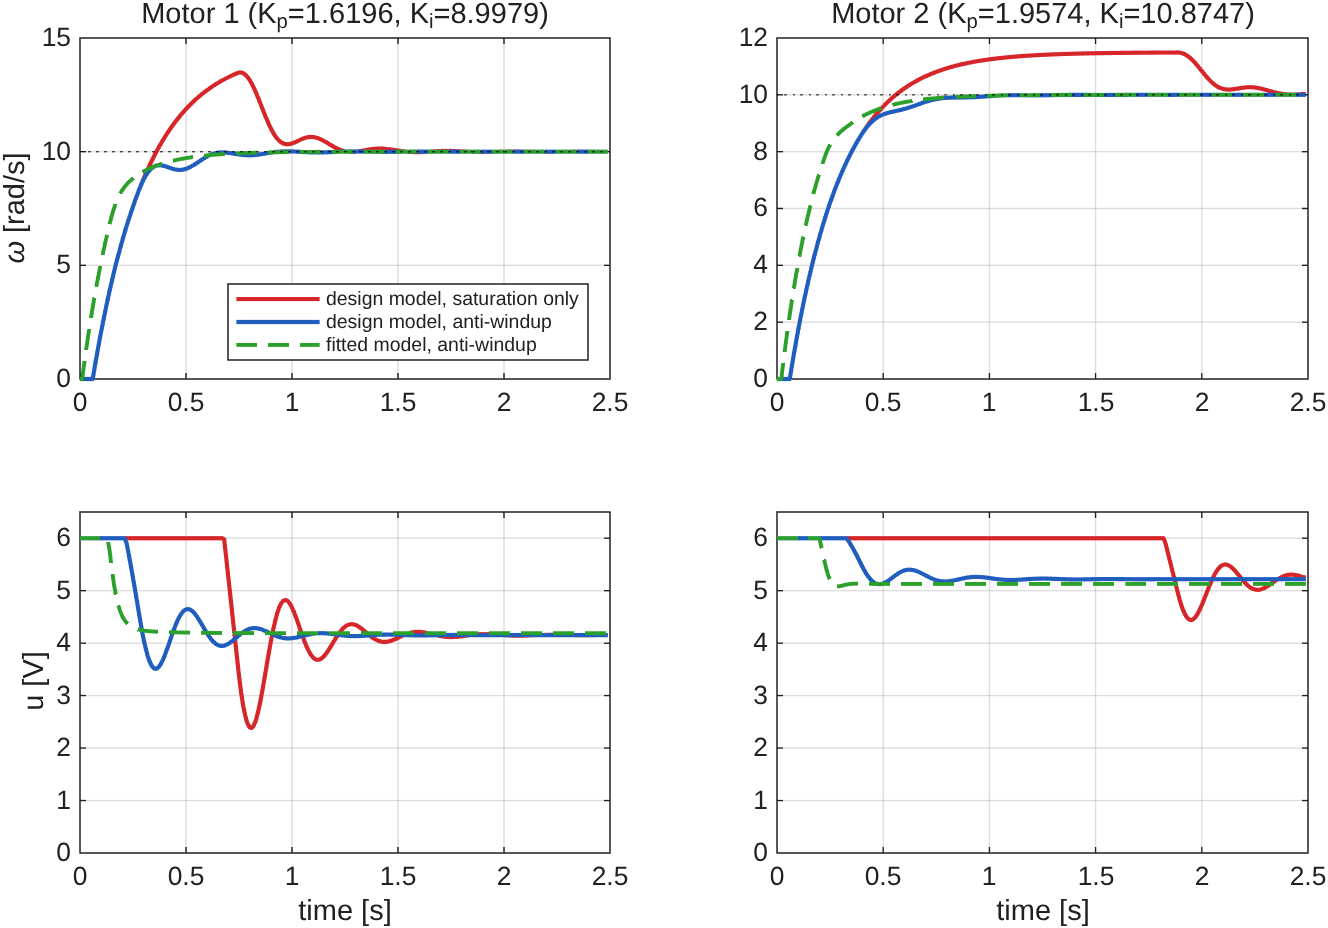
\includegraphics[width=0.85\textwidth]{figures/closed_loop_both.png}
  \caption{Simulated closed-loop response to a 10~rad/s step for both motors: speed (top) and control action
    (bottom), with plain saturation and with anti-windup on the design model, and with anti-windup on the fitted
    model.}
  \label{fig:lab2-closedloop}
\end{figure}

\noindent On the design model the Ziegler--Nichols gains give low margins (about $31^\circ$ and 4.4~dB), as expected
for this method: without saturation the step would have an overshoot of 65\,\%. With the 6~V limit, however, the
saturation dominates the transient. With plain saturation the integral winds up and the overshoot is 35\,\% for
motor~1; for motor~2, which needs 5.2~V in steady state, the output stays saturated for 1.8~s and the response settles
only after 2.3~s. With anti-windup both motors reach 10~rad/s without overshoot in 0.6--0.7~s, which is about half of
the open-loop settling time ($4T\approx1$~s), and the control action settles at $10/\mu$ (4.15~V and 5.2~V). On the
fitted model, which has less delay, the same gains give phase margins of $66$--$77^\circ$. Since the fitted model
should be closer to the real motors, we expect the real system to be at least as well damped as our simulation.
Among the versions we simulated, the PI with anti-windup gives the best response.

\subsection{Conclusions}

In this laboratory we identified both motors in open loop with an automatic sequence of five voltage steps. With the
63.2\,\% method on the filtered speed, the first-order model at the operating point $V_a=3.84$~V is
$\mu=2.41$~rad/s/V, $T=0.26$~s, $\tau=0.06$~s for motor~1 and $\mu=1.92$~rad/s/V, $T=0.25$~s, $\tau=0.06$~s for
motor~2: the two motors have similar dynamics, but the gain of motor~2 is about 20\,\% lower. The tangent method gave
the right order of magnitude but a time constant about 45\,\% larger, because it depends on the derivative, which is
sensitive both to the noise and to the delay of the filter. By fitting the model on the raw data we also found that
most of the identified delay was introduced by our filter: the real delay is about one sample and the real time
constant about 0.2~s.

Comparing the different recordings, we saw that brake mode is much closer to a linear system than coast mode, where
the gain is about twice as large and changes a lot with the amplitude, and that the gain in reverse is 20--25\,\%
lower than in forward. The gain also grows by about 25\,\% between 2~V and 6~V, so the linear model is valid only
around its operating point.

With Ziegler--Nichols we obtained $K_p=1.62$, $K_i=9.00$ for motor~1 and $K_p=1.96$, $K_i=10.87$ for motor~2. In
simulation the controller is fast, but the 6~V saturation causes integral wind-up; with an anti-windup based on
conditional integration both motors reach a 10~rad/s reference without overshoot in about 0.6--0.7~s. The most
important things we learned are how much the measurement chain (quantization, counter wrap-around, filtering)
affects the identification, and that the result of the identification must always be checked against the data.

\end{document}
